\chapter{Methodology}

This chapter presents our clustered federated deep reinforcement learning framework for chess with selective layer aggregation. We begin by formally defining the problem as an extension of the standard reinforcement learning formulation, incorporating the unique challenges of maintaining strategic diversity in a federated setting. We then describe the three-tier hierarchical aggregation system that enables knowledge transfer across clusters while preserving playstyle-specific characteristics. The chapter proceeds to detail the neural network architecture, the selective aggregation mechanism, the playstyle-aware data filtering strategy, and the complete training pipeline from supervised bootstrapping through self-play reinforcement learning. Finally, we present the evaluation methodology that will be used to validate our approach in Chapter 5.

\section{Problem Formulation}

This section establishes the formal mathematical framework for our clustered federated reinforcement learning approach to chess. We begin by formulating chess as a Markov Decision Process, then extend this formulation to incorporate the dual objectives of performance optimization and strategic diversity preservation within a federated learning setting.

\subsection{Markov Decision Process Formulation}

We formulate chess as a Markov Decision Process (MDP)~\cite{sutton2018reinforcement}, defined by the tuple $\mathcal{M} = (S, A, P, R, \gamma)$. The state space $S$ represents all possible board configurations, including piece positions, castling rights, en passant opportunities, and move history. Each state $s \in S$ encodes a complete chess position along with the relevant game state information required to determine legal moves. The action space $A(s)$ contains all legal moves available from state $s$, varying in size depending on the position but typically containing between 20 and 80 possible moves in non-trivial positions.

The transition function $P(s' | s, a)$ is deterministic in chess, as each legal move $a$ from state $s$ results in a unique next state $s'$. The reward function $R(s, a, s')$ provides feedback about the quality of moves and game outcomes. In our implementation, rewards are primarily assigned at terminal states, with $R = +1$ for winning positions, $R = -1$ for losing positions, and $R = 0$ for draws. The discount factor $\gamma \in [0, 1]$ determines the relative importance of immediate versus future rewards, though in chess with deterministic transitions to terminal states, this factor plays a less critical role than in many other RL domains.

The objective in the single-agent setting is to learn a policy $\pi: S \rightarrow A$ that maximizes the expected cumulative reward. In chess, this corresponds to finding a policy that maximizes win probability while minimizing loss probability across all possible game trajectories. The policy is typically parameterized by a neural network with parameters $\theta$, yielding $\pi_\theta(a|s)$, which outputs a probability distribution over legal actions given the current state.

\subsection{Strategic Diversity Objective}

Traditional federated learning~\cite{mcmahan2017communication} aims to train a single global model by aggregating knowledge from distributed clients. However, our framework introduces a fundamentally different objective: we seek to train multiple distinct models, each specialized for a different strategic approach to chess, while still enabling beneficial knowledge transfer between them. This dual objective creates a tension between convergence and divergence that standard federated learning algorithms are not designed to handle.

Formally, we partition our set of $N$ clients into $K$ clusters $C_1, C_2, \ldots, C_K$, where each cluster $C_k$ is associated with a distinct playstyle characteristic. In our primary experiments, we focus on $K=2$ clusters representing tactical and positional playing styles. Each cluster maintains its own cluster-specific model with parameters $\theta_k$, rather than converging to a single shared model $\theta_{\text{global}}$ as in standard federated learning.

The strategic diversity objective can be expressed as a bi-objective optimization problem. First, we seek to maximize the performance of each cluster-specific model on its designated playstyle:
\begin{equation}
\max_{\theta_k} \mathbb{E}_{s,a \sim \pi_{\theta_k}} [R(s,a)] \quad \forall k \in \{1, \ldots, K\}
\end{equation}

Second, we aim to maintain measurable divergence between cluster models, ensuring that strategic specialization is preserved:
\begin{equation}
\text{Divergence}(\theta_i, \theta_j) \geq \delta_{\min} \quad \forall i \neq j
\end{equation}
where $\delta_{\min}$ represents a minimum threshold for model differentiation, and the divergence metric can be quantified through various measures such as L2 distance between model parameters, distributional differences in move selection, or behavioral metrics like move type distributions.

This formulation differs fundamentally from standard federated learning, where the objective is typically $\min_\theta \sum_{i=1}^N \mathcal{L}_i(\theta)$, seeking a single $\theta$ that minimizes the aggregate loss across all clients. Instead, we seek a set of parameters $\{\theta_1, \ldots, \theta_K\}$ that balance individual cluster performance with cross-cluster knowledge transfer while maintaining strategic differentiation.

\subsection{Federated Learning Constraints}

Our problem formulation must satisfy several constraints inherent to federated learning systems. The privacy preservation constraint requires that raw training data remains local to each client. Clients train on their own datasets $D_i$ and only share model parameters or gradients with the central server, never exposing individual game records or training examples. This constraint is particularly relevant in scenarios where training data might contain proprietary opening preparation or game analysis.

The communication efficiency constraint limits the frequency and size of model updates transmitted between clients and the server. Let $T$ denote the total number of training rounds and $B$ the bandwidth available per round. Each communication round $t$ involves clients uploading local model parameters and downloading aggregated cluster models, with total communication cost proportional to the model size and number of participating clients. We denote the communication cost per round as $C_{\text{comm}}(t)$ and require $\sum_{t=1}^T C_{\text{comm}}(t) \leq B \cdot T$.

The heterogeneity constraint acknowledges that clients may have different computational capabilities, data distributions, and training objectives. Unlike traditional federated learning settings~\cite{li2020federated} that treat heterogeneity as an obstacle to convergence, our framework explicitly leverages this heterogeneity to maintain strategic diversity. Clients within cluster $C_k$ train on data that emphasizes playstyle $k$, creating non-IID data distributions across clusters by design.

Finally, the asynchronous participation constraint allows clients to join and leave training rounds dynamically. Not all clients participate in every round, and we denote the set of participating clients in round $t$ as $S_t \subseteq \{1, \ldots, N\}$. The aggregation mechanism must be robust to varying participation rates while ensuring that each cluster maintains sufficient representation in each training round.

\subsection{Performance Metrics}

Evaluating our framework requires metrics that capture both playing strength and strategic diversity. We organize our metrics into three categories: performance metrics, model-level divergence metrics, and behavioral metrics.

For playing strength evaluation, we employ ELO rating estimation through systematic matches against the Stockfish chess engine at multiple difficulty levels. Each cluster model is evaluated independently, producing separate ELO estimates $\text{ELO}_k$ for each cluster $k$, along with confidence intervals based on rating deviation. This allows us to assess whether selective layer sharing improves playing strength compared to fully independent training or complete parameter sharing, and whether both clusters maintain competitive performance despite their specialization.

Strategic diversity at the model level is quantified through cluster divergence metrics that examine the internal representations learned by different cluster models. For each layer $\ell$ in the network, we compute the cosine similarity between corresponding weight tensors $\theta_k^\ell$ and $\theta_j^\ell$ from clusters $k$ and $j$, defined as $\cos(\theta_k^\ell, \theta_j^\ell) = \frac{\theta_k^\ell \cdot \theta_j^\ell}{\|\theta_k^\ell\|_2 \|\theta_j^\ell\|_2}$. We also compute the normalized L2 distance $d_\ell(\theta_k, \theta_j) = \frac{\|\theta_k^\ell - \theta_j^\ell\|_2}{\sqrt{\|\theta_k^\ell\|_2^2 + \|\theta_j^\ell\|_2^2}}$ to capture magnitude differences. These layer-wise metrics are aggregated into group-level divergence scores for the input block, early residual layers, middle residual layers, late residual layers, policy head, and value head. This hierarchical analysis reveals which network components remain shared across clusters and which become specialized.

Weight statistics complement divergence metrics by tracking the evolution of model parameters during training. For each cluster and layer group, we monitor the mean, standard deviation, minimum, and maximum weight values, as well as the proportion of weights near zero. This helps identify potential training issues such as vanishing gradients, dead neurons, or unstable optimization. We also track the magnitude of weight changes between consecutive rounds, quantifying the learning rate and convergence behavior at different network depths.

Behavioral diversity is assessed through playstyle evaluation and move type distribution analysis. The playstyle score $\psi(M)$ for a model $M$ combines multiple chess-specific metrics derived from self-play games. Following the methodology of Novachess.ai, we analyze attacked material, legal move counts, material captured, and center control during the critical middle-game phase. These metrics are normalized and combined through a weighted average to produce a tactical score ranging from 0 (very positional) to 1 (very tactical), with intermediate values indicating balanced play. The classification provides both a continuous score and discrete categories ranging from very positional through balanced to very tactical.

Move type distribution metrics provide a complementary behavioral perspective by classifying each move in self-play games into categories: captures, checks, pawn advances, piece development, castling, quiet moves, and aggressive moves (captures plus checks). For each cluster, we compute the percentage of moves falling into each category, averaged across multiple games. Let $P_k(m)$ denote the empirical probability that cluster $k$ plays move type $m$. The difference in move type distributions between clusters, measured as $\Delta_{\text{aggressive}} = P_{\text{tactical}}(\text{captures}) + P_{\text{tactical}}(\text{checks}) - P_{\text{positional}}(\text{captures}) - P_{\text{positional}}(\text{checks})$, quantifies whether tactical clusters genuinely exhibit more forcing, aggressive play compared to positional clusters.

These metrics collectively enable us to assess whether our selective aggregation strategy successfully balances the competing objectives of performance optimization through knowledge sharing and strategic diversity preservation through cluster-specific specialization. The empirical validation of our approach requires demonstrating that intermediate sharing strategies achieve superior performance and diversity compared to the baseline extremes of complete sharing or complete independence, while maintaining measurable divergence in both model parameters and behavioral characteristics.

\section{Clustered Federated Learning Framework}

This section describes the overall architecture of our clustered federated learning system for chess. We present the high-level framework design, explain the rationale for our cluster organization, detail the client-server infrastructure, and specify the communication protocols that enable distributed training.

\subsection{Framework Overview}

Our clustered federated learning framework extends traditional federated learning by introducing multiple cluster-specific models rather than a single global model. The system consists of a central aggregation server and a distributed set of training clients organized into playstyle-based clusters. Unlike standard federated averaging, where all clients contribute to a unified global model, our framework maintains separate models for each cluster while enabling selective knowledge transfer between them.

The framework operates through three hierarchical levels of aggregation. At the lowest level, individual clients perform local training through self-play reinforcement learning, generating training experiences and updating their local model parameters. At the intermediate level, clients within the same cluster periodically synchronize their models through standard federated averaging, creating a cluster-specific model that captures the shared knowledge of that playstyle group. At the highest level, selective inter-cluster aggregation shares specific layers across clusters while keeping others cluster-specific, enabling knowledge transfer of fundamental chess understanding without homogenizing strategic preferences.

Figure~\ref{fig:system-architecture} illustrates the overall system architecture. The central server coordinates training across multiple distributed clients, which are organized into tactical and positional clusters. Each cluster maintains its own model, and the selective aggregation mechanism enables controlled knowledge sharing between clusters while preserving their distinct characteristics.

\begin{figure}[htbp]
\centering
\begin{tikzpicture}[
    scale=1,
    transform shape,
    node distance=1cm,
    client/.style={rectangle, draw=black, fill=blue!20, minimum width=1cm, minimum height=0.6cm, font=\scriptsize},
    server/.style={rectangle, draw=black, fill=green!20, minimum width=2.5cm, minimum height=1cm, font=\small},
    cluster/.style={rectangle, draw=black, dashed, line width=0.8pt, minimum width=4.5cm, minimum height=3.2cm},
    arrow/.style={->, >=stealth, thick}
]

% Server at top
\node[server] (server) at (0, 0) {Aggregation Server};

% Tactical Cluster (left)
\node[cluster] (tactical-box) at (-4, -3.8) {};
\node[font=\small] at (-5, -2.0) {\textbf{Tactical Cluster}};

% Tactical clients centered in cluster
\node[client, fill=red!20] (t1) at (-4.8, -3.2) {T1};
\node[client, fill=red!20] (t2) at (-3.2, -3.2) {T2};
\node[client, fill=red!20] (t3) at (-4.8, -4.2) {T3};
\node[client, fill=red!20] (t4) at (-3.2, -4.2) {T4};
\node[font=\footnotesize, below=0.1cm of tactical-box] {$\theta_{\text{tactical}}$};

% Positional Cluster (right)
\node[cluster] (positional-box) at (4, -3.8) {};
\node[font=\small] at (5, -2.0) {\textbf{Positional Cluster}};

% Positional clients centered in cluster
\node[client, fill=blue!20] (p1) at (3.2, -3.2) {P1};
\node[client, fill=blue!20] (p2) at (4.8, -3.2) {P2};
\node[client, fill=blue!20] (p3) at (3.2, -4.2) {P3};
\node[client, fill=blue!20] (p4) at (4.8, -4.2) {P4};
\node[font=\footnotesize, below=0.1cm of positional-box] {$\theta_{\text{positional}}$};

% Upload arrows (dashed, from clients to server)
\draw[->, >=stealth, red!70, dashed, line width=1pt] (t1) -- (-1.5, -1.2) -- (server);
\draw[->, >=stealth, red!70, dashed, line width=1pt] (t2) -- (-1.5, -1.2) -- (server);
\draw[->, >=stealth, red!70, dashed, line width=1pt] (t3) -- (-1.5, -1.2) -- (server);
\draw[->, >=stealth, red!70, dashed, line width=1pt] (t4) -- (-1.5, -1.2) -- (server);

\draw[->, >=stealth, blue!70, dashed, line width=1pt] (p1) -- (1.5, -1.2) -- (server);
\draw[->, >=stealth, blue!70, dashed, line width=1pt] (p2) -- (1.5, -1.2) -- (server);
\draw[->, >=stealth, blue!70, dashed, line width=1pt] (p3) -- (1.5, -1.2) -- (server);
\draw[->, >=stealth, blue!70, dashed, line width=1pt] (p4) -- (1.5, -1.2) -- (server);

% Download arrows (solid, from server to clients)
\draw[->, >=stealth, red!70, solid, line width=1pt] (server) -- (-1.5, -1.2) -- (t1);
\draw[->, >=stealth, red!70, solid, line width=1pt] (server) -- (-1.5, -1.2) -- (t2);
\draw[->, >=stealth, red!70, solid, line width=1pt] (server) -- (-1.5, -1.2) -- (t3);
\draw[->, >=stealth, red!70, solid, line width=1pt] (server) -- (-1.5, -1.2) -- (t4);

\draw[->, >=stealth, blue!70, solid, line width=1pt] (server) -- (1.5, -1.2) -- (p1);
\draw[->, >=stealth, blue!70, solid, line width=1pt] (server) -- (1.5, -1.2) -- (p2);
\draw[->, >=stealth, blue!70, solid, line width=1pt] (server) -- (1.5, -1.2) -- (p3);
\draw[->, >=stealth, blue!70, solid, line width=1pt] (server) -- (1.5, -1.2) -- (p4);

% Inter-cluster selective sharing arrow
\draw[->, >=stealth, thick, purple, <->, line width=1.2pt] (-1.2, -5.2) -- node[above, font=\scriptsize] {Selective Sharing} (1.2, -5.2);

\end{tikzpicture}
\caption{System architecture showing the central aggregation server coordinating two clusters of distributed clients. Tactical cluster clients (red) and positional cluster clients (blue) upload model updates to the server and download cluster-specific models. Selective inter-cluster aggregation enables knowledge transfer between clusters.}
\label{fig:system-architecture}
\end{figure}

This hierarchical design addresses the core challenge of balancing collaboration and specialization. By aggregating within clusters, we enable efficient knowledge sharing among clients with similar objectives. By selectively sharing across clusters, we transfer generalizable representations while maintaining cluster-specific strategic characteristics. The result is a system that leverages the full training data across all clients while producing multiple distinct models optimized for different playing styles.

\subsection{Cluster Design}

We organize clients into two primary clusters based on chess playstyle: tactical and positional. This binary clustering reflects a fundamental dichotomy in chess strategy that has persisted throughout the game's history. Tactical players prioritize concrete calculation, forcing moves, and immediate threats. Positional players emphasize long-term strategic planning, structural advantages, and prophylactic thinking. While these represent endpoints on a spectrum, they provide a clear organizational principle for cluster assignment and a testable hypothesis about strategic diversity preservation.

The tactical cluster trains primarily on sharp, forcing positions with concrete tactical themes. Training data for this cluster is filtered to emphasize openings with early confrontation, games featuring high capture rates, and tactical puzzles requiring precise calculation. The positional cluster trains on strategic positions with long-term planning requirements. Filtered data includes solid openings with emphasis on structure, games with lower exchange rates, and positional puzzles focusing on prophylaxis and planning.

Cluster assignment follows a semi-supervised approach. Initial assignment uses playstyle scores computed from each client's early training games, placing clients into clusters based on their observed tactical tendencies. However, cluster membership is not fixed. Every 20 training rounds, we recompute playstyle scores and allow clients to migrate between clusters if their playing style has shifted significantly. This dynamic reassignment handles the evolution of client behavior during training while maintaining sufficient stability for meaningful cluster-specific learning.

The decision to use two clusters rather than a larger number balances several considerations. Two clusters provide clear interpretability and testability for our core hypotheses about diversity preservation. The tactical-positional dichotomy has well-established foundations in chess theory, making results easier to validate and interpret. Computational overhead scales with the number of clusters, and two clusters allow us to thoroughly evaluate the selective aggregation mechanism without excessive resource requirements. Future work could extend the framework to finer-grained clustering schemes, such as organizing clients by specific opening repertoires or endgame specializations.

\subsection{Client-Server Architecture}

The distributed system architecture follows a star topology with a central aggregation server coordinating multiple training clients. The server maintains authoritative copies of cluster-specific models, orchestrates training rounds, aggregates client updates, and distributes updated models. Clients perform local training through self-play, compute model updates, and communicate with the server to exchange parameters.

Each training round proceeds through a well-defined protocol. The server first selects a subset of participating clients for the current round, ensuring balanced representation from each cluster. Selected clients download the current cluster-specific model corresponding to their assigned cluster. Clients then perform local training for a fixed number of epochs, generating self-play games, collecting training experiences, and updating model parameters through stochastic gradient descent. After completing local training, clients upload their updated model parameters to the server.

The server collects updates from all participating clients and performs aggregation at two levels. First, intra-cluster aggregation computes the weighted average of model parameters within each cluster, where weights typically correspond to the number of training examples processed by each client. This produces updated cluster-specific models that incorporate the collective knowledge of all participating clients in each cluster. Second, selective inter-cluster aggregation shares specified layers across clusters through federated averaging while leaving other layers cluster-specific. The server then stores the updated models and metrics, and the process repeats for the next round.

This architecture provides several advantages over fully peer-to-peer alternatives. Centralized aggregation simplifies coordination and ensures consistent model versions across clients. The server can implement sophisticated aggregation strategies that would be difficult to coordinate in a decentralized setting. Fault tolerance is enhanced, as individual client failures do not disrupt the overall training process. The architecture also facilitates monitoring and evaluation, with the server maintaining comprehensive logs of training metrics and model checkpoints.

\subsection{Communication Protocol}

Communication between clients and the server follows an asynchronous protocol that balances training efficiency with network constraints. The protocol is designed to minimize communication overhead while ensuring that aggregation occurs frequently enough to enable effective knowledge transfer.

Model transmission uses parameter differencing to reduce bandwidth requirements. Rather than transmitting full model parameters each round, clients compute and transmit only the difference between their locally updated model and the initial model they downloaded. For a parameter vector $\theta_{\text{new}}$ after local training and initial parameters $\theta_{\text{old}}$, the client transmits $\Delta\theta = \theta_{\text{new}} - \theta_{\text{old}}$. The server reconstructs updated parameters as $\theta_{\text{new}} = \theta_{\text{old}} + \Delta\theta$. This significantly reduces transmission size, particularly in early training rounds when parameter changes are small.

The protocol handles network unreliability through timeout mechanisms and retry logic. Clients set a maximum time limit for upload and download operations. If a client fails to receive an acknowledgment within the timeout period, it retries the transmission up to a maximum number of attempts. If all attempts fail, the client skips the current round and attempts to rejoin in the next round. The server similarly implements timeouts when waiting for client uploads, proceeding with aggregation using only the subset of clients that successfully transmitted their updates.

Synchronization between training rounds follows a flexible schedule that accommodates varying client availability. The server does not require all clients to participate in every round. Instead, it waits for a minimum threshold of clients from each cluster before proceeding with aggregation. This minimum threshold ensures that cluster-specific models benefit from sufficient data diversity while allowing training to proceed even when some clients are offline. If the threshold is not met within a specified time window, the server proceeds with aggregation using available clients, though this situation is logged for monitoring purposes.

Security and privacy considerations are addressed through parameter-level aggregation rather than data sharing. Clients never transmit raw training games or board positions to the server. All communication consists solely of model parameters or parameter differences, which do not directly reveal individual training examples. While sophisticated attacks could potentially extract some information from parameter updates, the aggregation of multiple client updates provides a degree of privacy protection similar to standard federated learning systems.

\section{Neural Network Architecture}
\label{sec:network-architecture}

This section describes the deep neural network architecture used by all agents in our federated learning framework. We employ an AlphaZero-style convolutional residual network that takes board positions as input and produces dual outputs: a policy distribution over legal moves and a scalar value estimation. The architecture is designed to support selective layer aggregation, with distinct functional groups that can be shared across clusters or maintained cluster-specifically (see Figure~\ref{fig:network-architecture}). We detail the input representation, the residual network structure, the dual output heads, and the layer grouping scheme that enables our selective aggregation strategy.

\subsection{Input Representation}

The neural network receives chess positions as a structured tensor representation encoding the board state, game rules, and move history. Rather than using a simple 8×8 grid with piece identifiers, we employ a rich multi-plane encoding that provides the network with comprehensive positional information while maintaining spatial structure.

The input tensor has shape $8 \times 8 \times 119$, representing 119 feature planes over the standard chessboard grid (Figure~\ref{fig:network-architecture}). The first 12 planes encode the current piece positions using one-hot encoding, with separate planes for each piece type and color: white pawns, white knights, white bishops, white rooks, white queens, white king, and the corresponding black pieces. Each plane is a binary matrix where a 1 indicates the presence of that piece type at the corresponding square.

To provide temporal context, we include piece positions from the previous seven board states, using an additional 84 planes (12 planes per historical position × 7 time steps). This history enables the network to recognize repetitions, understand pawn structure changes, and track piece mobility patterns across recent moves. The historical encoding is essential for positions where the optimal move depends on the sequence of preceding moves rather than the current position alone.

The remaining 23 planes encode game state information that cannot be inferred from piece positions alone. One plane indicates whose turn it is to move, with all squares set to 1 for white to move and 0 for black to move. Four planes encode castling rights, with separate planes for white kingside, white queenside, black kingside, and black queenside castling availability. One plane marks en passant target squares when applicable. The final 17 planes encode the halfmove clock using a thermometer encoding, representing the number of moves since the last pawn advance or capture, which is critical for the fifty-move rule.

This 119-plane representation provides the network with complete information about the position while preserving the 2D spatial structure of the board. Convolutional layers can exploit translational patterns across the board, learning features that apply regardless of whether a tactical pattern appears on the kingside or queensside. The representation is compatible with the standard AlphaZero approach while containing all information necessary to determine legal moves and evaluate positions according to chess rules.

\subsection{Residual Network Structure}

Following the input representation, the network applies an initial convolution block to transform the 119 input planes into a higher-dimensional feature space. This input convolution consists of a $3 \times 3$ convolutional layer with 256 output channels, followed by batch normalization and a ReLU activation function. The use of 256 channels provides sufficient representational capacity for the network to learn rich feature representations while remaining computationally tractable for distributed training across multiple clients.

The core of the architecture consists of 19 residual blocks, each implementing the standard residual connection pattern introduced by He et al. Each residual block contains two $3 \times 3$ convolutional layers with 256 channels, with batch normalization and ReLU activation applied after each convolution. The residual connection adds the block's input directly to its output before the final activation, enabling gradient flow through the deep network and facilitating the learning of incremental refinements to the feature representation.

The choice of 19 residual blocks balances network depth with training efficiency. Deeper networks can learn more sophisticated positional patterns but require more computational resources and training data. Our 19-block configuration matches the architecture scale used in moderate-strength AlphaZero implementations and proves sufficient for learning chess at an advanced amateur level. Each block operates on $8 \times 8 \times 256$ feature maps, progressively refining the internal representation through the depth of the network.

The residual blocks are grouped functionally into three categories based on their position in the network: early blocks (blocks 1-6), middle blocks (blocks 7-13), and late blocks (blocks 14-19), as shown in Figure~\ref{fig:network-architecture}. This grouping reflects the hierarchical nature of feature learning in deep networks. Early blocks tend to learn low-level spatial patterns and piece configurations. Middle blocks learn tactical motifs and multi-piece coordination. Late blocks integrate high-level strategic concepts and complex positional evaluations. This functional division becomes important for our selective aggregation strategy, as different layer groups may benefit differently from cross-cluster sharing.
\subsection{Policy and Value Heads}

After the 19 residual blocks, the feature representation branches into two separate output heads: a policy head that predicts move probabilities and a value head that estimates position evaluation (Figure~\ref{fig:network-architecture}). This dual-head architecture enables the network to learn both which moves to consider and how to evaluate the resulting positions, supporting the Monte Carlo Tree Search algorithm used during move selection.

The policy head transforms the $8 \times 8 \times 256$ feature maps into a probability distribution over possible moves. It consists of a $1 \times 1$ convolution that reduces the channel dimension from 256 to 2, followed by batch normalization and ReLU activation. The resulting $8 \times 8 \times 2$ tensor is flattened to a vector of length 128, which is then passed through a fully connected layer with 4672 output units. This output dimension corresponds to the maximum number of possible chess moves in the standard representation: 64 source squares × 73 possible destination patterns (including underpromotions and all move types). A softmax activation produces the final policy distribution $\pi$, with illegal moves masked to zero probability based on the current position.

The value head estimates the expected outcome from the current position. It applies a $1 \times 1$ convolution to reduce the channel dimension from 256 to 1, followed by batch normalization and ReLU activation. The resulting $8 \times 8 \times 1$ tensor is flattened to a 64-dimensional vector and passed through a fully connected layer with 256 hidden units and ReLU activation. A final fully connected layer with a single output unit, followed by a tanh activation, produces the value estimation $v \in [-1, 1]$, where -1 represents a certain loss, +1 represents a certain win, and 0 represents an even position.

Both heads are trained simultaneously using a combined loss function. The policy head is trained with cross-entropy loss against the improved policy distribution produced by MCTS during self-play, encouraging the network to predict the same moves that tree search identifies as strong. The value head is trained with mean squared error against the actual game outcomes, learning to predict position evaluation directly. The dual-head design shares the representational work of the residual tower while specializing the final layers for their distinct prediction tasks.
\subsection{Layer Grouping for Selective Aggregation}

To enable selective parameter sharing in our federated learning framework, we partition the neural network into functionally distinct layer groups. Each group represents a coherent set of parameters that can be independently chosen for cluster-specific or cross-cluster aggregation. This grouping reflects both the hierarchical structure of the network and the hypothesis that different layers may benefit differently from exposure to diverse playing styles.

We define five layer groups (Figure~\ref{fig:network-architecture}). The \textbf{input block} comprises the initial $3 \times 3$ convolutional layer, batch normalization, and activation that transforms the 119-plane input representation into 256-channel feature maps. This group contains the parameters that process raw board encodings into a learned feature space. The \textbf{early residual blocks} group includes residual blocks 1 through 6, which learn fundamental spatial patterns and piece relationships. The \textbf{middle residual blocks} group contains blocks 7 through 13, which learn tactical patterns and multi-piece coordination. The \textbf{late residual blocks} group encompasses blocks 14 through 19, which integrate strategic concepts and high-level position evaluation.

The final two groups separate the output heads. The \textbf{policy head} group contains all parameters involved in move prediction, including the policy-specific convolution, fully connected layers, and softmax activation. The \textbf{value head} group contains all parameters for position evaluation, including the value-specific convolution, hidden layer, and final value output. This separation allows independent decisions about whether move selection patterns and position evaluation should be shared across playstyle clusters.

This five-group partition provides sufficient granularity to test hypotheses about which network components benefit from cross-cluster knowledge transfer. Early layers that learn universal chess patterns might benefit from aggregation across all clients regardless of playstyle. Middle and later layers that encode tactical and strategic preferences might require cluster-specific aggregation to preserve distinct playing styles. The policy and value heads might show different sensitivity to cross-cluster aggregation, as move preferences may be more playstyle-dependent than outcome predictions. The grouping enables these hypotheses to be tested empirically through controlled experiments with different selective aggregation configurations.

\begin{figure}[htbp]
\centering
\begin{tikzpicture}[
    scale=1,
    transform shape,
    node distance=0.3cm,
    layer/.style={rectangle, draw=black, fill=blue!10, minimum width=4cm, minimum height=0.7cm, font=\small},
    blockgroup/.style={rectangle, draw=black, fill=orange!15, minimum width=4cm, minimum height=1.8cm, font=\small, align=center},
    head/.style={rectangle, draw=black, fill=green!15, minimum width=1.8cm, minimum height=0.8cm, font=\small},
    annotation/.style={font=\scriptsize, text width=3.5cm, align=left},
    arrow/.style={->, >=stealth, thick}
]

% Input layer
\node[layer, fill=gray!20] (input) at (0, 0) {Input: $8 \times 8 \times 119$};

% Input block
\node[layer, fill=purple!15, below=of input] (input-conv) {Input Conv Block};
\node[annotation, right=0.8cm of input-conv] (input-ann) {3×3 conv, 256 channels\\BatchNorm, ReLU};

% Early residual blocks
\node[blockgroup, below=of input-conv] (early) {Early Residual Blocks\\(Blocks 1-6)};
\node[annotation, right=0.8cm of early] (early-ann) {\textbf{Group 1}\\Spatial patterns\\Shared};

% Middle residual blocks
\node[blockgroup, below=of early] (middle) {Middle Residual Blocks\\(Blocks 7-13)};
\node[annotation, right=0.8cm of middle] (middle-ann) {\textbf{Group 2}\\Tactical motifs\\Cluster-specific};

% Late residual blocks
\node[blockgroup, below=of middle] (late) {Late Residual Blocks\\(Blocks 14-19)};
\node[annotation, right=0.8cm of late] (late-ann) {\textbf{Group 3}\\Strategic concepts\\Cluster-specific};

% Branching point
\node[below=0.5cm of late] (branch) {};

% Policy head
\node[head, below left=0.5cm and 1cm of branch] (policy) {Policy Head};
\node[annotation, anchor=east, text width=2.2cm] at ([xshift=-0.2cm]policy.west) {\textbf{Group 4}\\$\pi$: move probs\\Cluster-specific};

% Value head
\node[head, below right=0.5cm and 1cm of branch] (value) {Value Head};
\node[annotation, right=0.3cm of value] (value-ann) {\textbf{Group 5}\\$v \in [-1,1]$\\Cluster-specific};

% Arrows
\draw[arrow] (input) -- (input-conv);
\draw[arrow] (input-conv) -- (early);
\draw[arrow] (early) -- (middle);
\draw[arrow] (middle) -- (late);
\draw[arrow] (late) -- (branch.center);
\draw[arrow] (branch.center) -| (policy);
\draw[arrow] (branch.center) -| (value);

% Legend for aggregation strategy
\node[draw, dashed, thick, fill=yellow!10, text width=4cm, font=\scriptsize, below=1.2cm of policy, xshift=2cm] (legend) {
\textbf{Aggregation Strategy:}\\
\textcolor{blue}{Shared}: Cross-cluster\\
\textcolor{red}{Cluster-specific}: Within-cluster
};

\end{tikzpicture}
\caption{Neural network architecture showing the input layer, residual tower with 19 blocks grouped into early, middle, and late stages, and dual output heads for policy and value prediction. Annotations indicate the five layer groups used for selective aggregation, with example aggregation strategies shown (shared for early layers, cluster-specific for middle and late layers and output heads).}
\label{fig:network-architecture}
\end{figure}


\section{Three-Tier Aggregation System}
\label{sec:aggregation-system}

Our federated learning framework employs a three-tier hierarchical aggregation mechanism that progressively combines knowledge from individual clients to cluster-specific models to cross-cluster shared representations. This hierarchical approach balances the benefits of distributed learning with the need to preserve playstyle-specific characteristics within each cluster. The three tiers operate at different frequencies and scopes: local training occurs continuously at each client, intra-cluster aggregation periodically combines updates within each playstyle cluster, and inter-cluster selective aggregation occasionally shares specific layer groups across clusters. Figure~\ref{fig:aggregation-flow} illustrates the complete aggregation pipeline and the flow of information through the three tiers.

\begin{figure}[htbp]
\centering
\begin{tikzpicture}[
    scale=1,
    transform shape,
    node distance=0.8cm,
    tier/.style={rectangle, draw=black, thick, fill=blue!10, minimum width=9cm, minimum height=2cm, font=\small, align=center},
    process/.style={rectangle, draw=black, fill=orange!20, minimum width=3cm, minimum height=0.8cm, font=\footnotesize},
    client/.style={rectangle, draw=black, fill=green!15, minimum width=1.5cm, minimum height=0.6cm, font=\scriptsize},
    arrow/.style={->, >=stealth, thick},
    label/.style={font=\small\bfseries}
]

% Tier 3: Inter-cluster (top)
\node[tier, fill=purple!10] (tier3) at (0, 0) {
    \textbf{Tier 3: Inter-Cluster Selective Aggregation}\\[0.2cm]
    Selective layer sharing across clusters\\
    Frequency: Every $M$ intra-cluster rounds
};

% Tier 2: Intra-cluster (middle)
\node[tier, fill=blue!10, below=1.2cm of tier3] (tier2) {
    \textbf{Tier 2: Intra-Cluster Aggregation}\\[0.2cm]
    FedAvg within each cluster\\
    Frequency: Every $K_{\text{intra}}$ games
};

% Tier 1: Local training (bottom)
\node[tier, fill=green!10, below=1.2cm of tier2] (tier1) {
    \textbf{Tier 1: Local Training}\\[0.2cm]
    Supervised bootstrapping + Self-play with MCTS\\
    Frequency: Continuous
};

% Arrows between tiers - Tier 1 to Tier 2
\draw[arrow, thick, ->] ([xshift=-2cm]tier1.north) -- node[left, font=\scriptsize, align=center] {Upload\\parameters} ([xshift=-2cm]tier2.south);
\draw[arrow, thick, <-] ([xshift=2cm]tier1.north) -- node[right, font=\scriptsize, align=center] {Download\\aggregated} ([xshift=2cm]tier2.south);

% Arrows between tiers - Tier 2 to Tier 3
\draw[arrow, thick, ->] ([xshift=-2cm]tier2.north) -- node[left, font=\scriptsize, align=center] {Upload\\cluster models} ([xshift=-2cm]tier3.south);
\draw[arrow, thick, <-] ([xshift=2cm]tier2.north) -- node[right, font=\scriptsize, align=center] {Download\\shared layers} ([xshift=2cm]tier3.south);

% Client boxes below Tier 1 (centered)
\node[below=0.8cm of tier1] (client-anchor) {};
\node[client, fill=red!20, left=2.5cm of client-anchor] (t1) {\tiny T1};
\node[client, fill=red!20, right=0.3cm of t1] (t2) {\tiny T2};
\node[font=\scriptsize, right=0.3cm of t2] (tdots) {};
\node[client, fill=blue!20, right=0.5cm of tdots] (p1) {\tiny P1};
\node[client, fill=blue!20, right=0.3cm of p1] (p2) {\tiny P2};
\node[font=\scriptsize, right=0.3cm of p2] {};

% Cluster labels
\node[font=\scriptsize, above=0.1cm of t1, xshift=0.75cm] {Tactical};
\node[font=\scriptsize, above=0.1cm of p1, xshift=0.75cm] {Positional};

\end{tikzpicture}
\caption{Three-tier hierarchical aggregation system showing the flow of information from local client training through intra-cluster aggregation to inter-cluster selective sharing. Arrows indicate bidirectional communication between tiers, with clients uploading parameters and downloading aggregated models. The time scales reflect the hierarchical nature of the system, with local training running continuously and higher tiers executing progressively less frequently.}
\label{fig:aggregation-flow}
\end{figure}

\subsection{Local Training Phase}

At the base tier, each client independently trains its neural network through a two-phase approach: supervised bootstrapping followed by reinforcement learning through self-play. This local training phase generates the diverse experiences and parameter updates that will ultimately be aggregated across the federation.

Training begins with a supervised bootstrapping phase where clients learn from historical games and tactical puzzles filtered according to their cluster's playstyle. Tactical cluster clients train on games featuring aggressive openings and tactical puzzles emphasizing combinations, while positional cluster clients train on strategic games and positional puzzles. This phase provides a foundation of chess knowledge and playstyle-specific patterns before transitioning to self-play. The bootstrapping phase and data filtering mechanisms are detailed in Sections~\ref{sec:playstyle-filtering} and~\ref{sec:training-procedures}.

Once bootstrapped, clients transition to self-play reinforcement learning. Each client maintains a complete copy of the neural network and uses it to play games against itself. For each move, the client performs Monte Carlo Tree Search guided by the current network's policy and value predictions. The search explores promising move sequences by repeatedly selecting moves, expanding the search tree, evaluating positions with the neural network, and backpropagating values through visited nodes. After completing the search, the client selects a move based on the visit counts of root actions, which represents an improved policy over the raw network output.

Training data is generated from these self-play games. Each position encountered during a game is stored along with the improved policy distribution derived from MCTS visit counts and the final game outcome. After accumulating a batch of training positions, the client trains its network by minimizing a combined loss function. The policy loss uses cross-entropy between the network's policy output and the MCTS-improved policy. The value loss uses mean squared error between the network's value prediction and the actual game outcome. The combined loss is $L = L_{\text{policy}} + \lambda L_{\text{value}}$, where $\lambda$ balances the two objectives.

The local training phase continues for a fixed number of games or training steps before the client's updated parameters are transmitted to the aggregation server for intra-cluster aggregation. The complete training procedure, including MCTS parameters and experience replay mechanisms, is described in Section~\ref{sec:training-procedures}.
\subsection{Intra-Cluster Aggregation}

The second tier of aggregation combines parameter updates from clients within each playstyle cluster to create a cluster-specific global model. This intra-cluster aggregation preserves the specialized characteristics of each playstyle while leveraging the collective learning of multiple clients pursuing similar strategic goals.

When clients complete a local training phase, they transmit their updated model parameters to the central aggregation server. The server maintains separate aggregation contexts for each cluster, ensuring that tactical and positional clients do not directly share parameters at this stage. For each cluster, the server applies federated averaging to compute a weighted mean of client parameters. Let $\theta_i^{(t)}$ denote the parameters of client $i$ in cluster $c$ at aggregation round $t$, and let $n_i$ represent the number of training examples processed by client $i$ since the last aggregation. The cluster-specific aggregated parameters are computed as:

\begin{equation}
\theta_c^{(t+1)} = \frac{\sum_{i \in c} n_i \theta_i^{(t)}}{\sum_{i \in c} n_i}
\end{equation}

This weighted averaging gives greater influence to clients that have processed more training data, under the assumption that more training leads to better parameter estimates. The aggregation is applied uniformly across all layer groups at this stage, creating a complete cluster-specific model that represents the collective knowledge of all clients in that cluster.

After aggregation, the server distributes the updated cluster-specific model $\theta_c^{(t+1)}$ back to all clients in cluster $c$. Each client replaces its local parameters with the aggregated parameters and resumes local training from this synchronized state. This synchronization allows clients to benefit from the diverse experiences of other clients in their cluster while maintaining their specialized playstyle focus. The frequency of intra-cluster aggregation is determined by the aggregation scheduling policy described in Section~\ref{sec:aggregation-scheduling}.
\subsection{Inter-Cluster Selective Aggregation}

The third and highest tier of aggregation selectively shares knowledge across playstyle clusters. Unlike intra-cluster aggregation which combines all parameters, inter-cluster aggregation operates only on specific layer groups identified as benefiting from cross-cluster knowledge transfer. This selective approach enables the system to learn universal chess patterns while preserving cluster-specific strategic preferences.

Inter-cluster aggregation is controlled by a layer group selection policy that specifies which of the five layer groups (input block, early residual blocks, middle residual blocks, late residual blocks, policy head, value head) should be aggregated across clusters. Based on the hypothesis that early layers learn universal patterns while later layers encode playstyle-specific strategies, a typical configuration might designate the input block and early residual blocks for cross-cluster sharing while keeping middle blocks, late blocks, and output heads cluster-specific.

For each layer group designated for cross-cluster aggregation, the server computes a global average across all clusters. Let $\theta_{c,g}^{(t)}$ denote the parameters of layer group $g$ in cluster $c$ at inter-cluster aggregation round $t$. The cross-cluster aggregated parameters for group $g$ are:

\begin{equation}
\theta_g^{(t+1)} = \frac{\sum_{c} n_c \theta_{c,g}^{(t)}}{\sum_{c} n_c}
\end{equation}

where $n_c$ represents the total number of training examples processed by all clients in cluster $c$ since the last inter-cluster aggregation. This ensures that clusters contributing more training data have proportionally greater influence on the shared representation.

After computing the cross-cluster averaged parameters for selected layer groups, the server distributes these shared parameters back to all clusters. Each cluster's model is updated by replacing the parameters of shared layer groups with the cross-cluster averaged values, while keeping cluster-specific layer groups unchanged. This selective replacement maintains the architectural integrity of the network while enabling knowledge transfer for designated components.

Inter-cluster aggregation occurs less frequently than intra-cluster aggregation, as it represents a higher-level consolidation of knowledge. The reduced frequency also mitigates the risk of disrupting cluster-specific learning by limiting how often cross-cluster information is injected into specialized models. The specific timing and frequency are determined by the aggregation scheduling policy detailed in the next subsection.
\subsection{Aggregation Scheduling}
\label{sec:aggregation-scheduling}

The three aggregation tiers operate on different time scales to balance learning efficiency with communication overhead and model stability. The scheduling policy determines when each tier executes and coordinates the flow of information through the hierarchical system.

Local training at Tier 1 runs continuously, with each client playing self-play games and updating its neural network parameters through gradient descent. Clients operate asynchronously without waiting for other clients or the server. This continuous local training ensures that computation resources are fully utilized and that learning progresses without interruption.

Intra-cluster aggregation at Tier 2 occurs periodically when clients have accumulated sufficient local training progress. In our implementation, clients perform intra-cluster aggregation after every $K_{\text{intra}}$ self-play games, where $K_{\text{intra}}$ is a hyperparameter controlling the aggregation frequency. After completing $K_{\text{intra}}$ games, a client uploads its current parameters to the server and waits for the server to perform aggregation and return the updated cluster model. The client then resumes training with the aggregated parameters. This periodic synchronization prevents clients from diverging too far from the cluster's collective knowledge while allowing substantial local progress between synchronizations.

Inter-cluster aggregation at Tier 3 occurs less frequently, after every $M$ intra-cluster aggregation rounds, where $M > 1$. This reduced frequency reflects the fact that cross-cluster knowledge transfer involves higher-level patterns that evolve more slowly than cluster-specific learning. The ratio $M$ controls the balance between cluster specialization and cross-cluster knowledge sharing. Larger values of $M$ allow clusters to develop more distinct characteristics before sharing knowledge, while smaller values promote more frequent integration of universal patterns.

The scheduling policy creates a natural hierarchy of time scales: local training operates on the scale of individual games (minutes), intra-cluster aggregation operates on the scale of training batches (tens of games), and inter-cluster aggregation operates on the scale of multiple aggregation rounds (hundreds of games). This hierarchical timing allows the system to efficiently combine rapid local learning with periodic consolidation at increasing levels of abstraction.


\section{Selective Layer Aggregation}

The selective layer aggregation mechanism is the key innovation that enables our framework to balance universal chess knowledge with playstyle-specific strategies. Rather than applying uniform federated averaging across all network parameters, we partition the network into functional layer groups and selectively choose which groups to aggregate across clusters. This section details the layer sharing strategy, the algorithmic implementation, the knowledge transfer mechanisms, and the expected convergence properties.

Figure~\ref{fig:layer-sharing} illustrates how different layer groups are treated during inter-cluster aggregation, with shared layers receiving cross-cluster knowledge transfer while cluster-specific layers remain isolated. Figure~\ref{fig:sharing-configs} presents the experimental configurations we evaluate, showing different hypotheses about which layers benefit from sharing..

\begin{figure}[htbp]
\centering
\begin{tikzpicture}[
    scale=1,
    transform shape,
    node distance=0.25cm,
    layer/.style={rectangle, draw=black, minimum width=3.5cm, minimum height=0.6cm, font=\scriptsize},
    shared/.style={fill=green!30},
    tactical/.style={fill=red!20},
    positional/.style={fill=blue!20},
    arrow/.style={->, >=stealth, thick}
]

% Tactical cluster (left)
\node[font=\small\bfseries] at (-2.5, 0) {Tactical Cluster};
\node[layer, tactical, below=0.3cm] (t-value) at (-2.5, -0.3) {Value Head};
\node[layer, tactical, below=of t-value] (t-policy) {Policy Head};
\node[layer, tactical, below=of t-policy] (t-late) {Late Blocks (14-19)};
\node[layer, tactical, below=of t-late] (t-middle) {Middle Blocks (7-13)};
\node[layer, shared, below=of t-middle] (t-early) {Early Blocks (1-6)};
\node[layer, shared, below=of t-early] (t-input) {Input Block};

% Positional cluster (right)
\node[font=\small\bfseries] at (2.5, 0) {Positional Cluster};
\node[layer, positional, below=0.3cm] (p-value) at (2.5, -0.3) {Value Head};
\node[layer, positional, below=of p-value] (p-policy) {Policy Head};
\node[layer, positional, below=of p-policy] (p-late) {Late Blocks (14-19)};
\node[layer, positional, below=of p-late] (p-middle) {Middle Blocks (7-13)};
\node[layer, shared, below=of p-middle] (p-early) {Early Blocks (1-6)};
\node[layer, shared, below=of p-early] (p-input) {Input Block};

% Cross-cluster aggregation arrows for shared layers
\draw[arrow, green!60!black, <->, line width=1.5pt] (t-early.east) -- node[above, font=\tiny] {aggregated} (p-early.west);
\draw[arrow, green!60!black, <->, line width=1.5pt] (t-input.east) -- node[above, font=\tiny] {aggregated} (p-input.west);

% X marks for non-shared layers
\node[font=\Large, red] at (0, -0.9) {\texttimes};
\node[font=\Large, red] at (0, -1.7) {\texttimes};
\node[font=\Large, red] at (0, -2.5) {\texttimes};
\node[font=\Large, red] at (0, -3.3) {\texttimes};

% Legend
\node[draw, fill=white, text width=4cm, font=\scriptsize, below=0.5cm of t-input, xshift=2.5cm] {
\textbf{Legend:}\\
\colorbox{green!30}{\phantom{XX}} Shared across clusters\\
\colorbox{red!20}{\phantom{XX}} Tactical-specific\\
\colorbox{blue!20}{\phantom{XX}} Positional-specific
};

\end{tikzpicture}
\caption{Selective layer sharing visualization showing how different layer groups are treated during inter-cluster aggregation in the baseline configuration (B1). Green layers (input block and early residual blocks) are aggregated across clusters, receiving cross-cluster knowledge transfer. Red and blue layers (middle blocks, late blocks, and output heads) remain cluster-specific, preserving strategic preferences. Arrows indicate cross-cluster aggregation; X marks indicate isolated layers.}
\label{fig:layer-sharing}
\end{figure}

\begin{figure}[htbp]
\centering
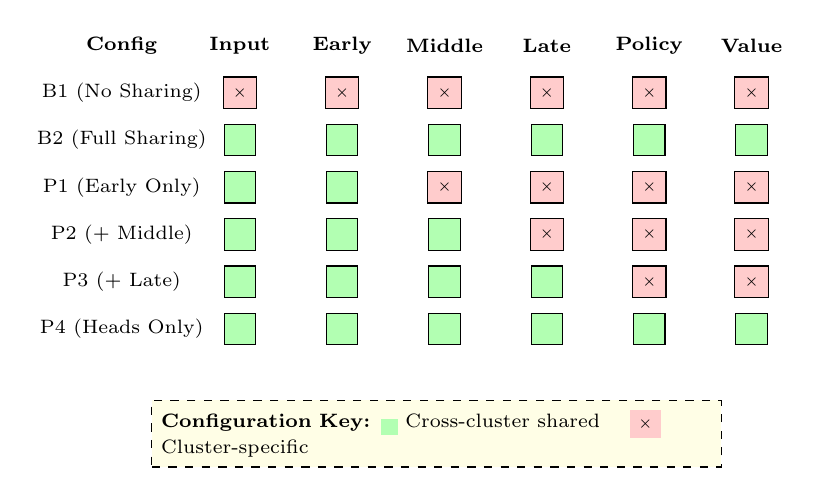
\begin{tikzpicture}[
    scale=1,
    transform shape
]

% Headers
\node[font=\scriptsize\bfseries] at (0, 0) {Config};
\node[font=\scriptsize\bfseries] at (1.5, 0) {Input};
\node[font=\scriptsize\bfseries] at (2.8, 0) {Early};
\node[font=\scriptsize\bfseries] at (4.1, 0) {Middle};
\node[font=\scriptsize\bfseries] at (5.4, 0) {Late};
\node[font=\scriptsize\bfseries] at (6.7, 0) {Policy};
\node[font=\scriptsize\bfseries] at (8, 0) {Value};

% Row labels
\node[font=\scriptsize] at (0, -0.6) {B1 (No Sharing)};
\node[font=\scriptsize] at (0, -1.2) {B2 (Full Sharing)};
\node[font=\scriptsize] at (0, -1.8) {P1 (Early Only)};
\node[font=\scriptsize] at (0, -2.4) {P2 (+ Middle)};
\node[font=\scriptsize] at (0, -3.0) {P3 (+ Late)};
\node[font=\scriptsize] at (0, -3.6) {P4 (Heads Only)};

% B1: No sharing (independent)
\node[draw, fill=red!20, minimum size=0.4cm] at (1.5, -0.6) {\tiny $\times$};
\node[draw, fill=red!20, minimum size=0.4cm] at (2.8, -0.6) {\tiny $\times$};
\node[draw, fill=red!20, minimum size=0.4cm] at (4.1, -0.6) {\tiny $\times$};
\node[draw, fill=red!20, minimum size=0.4cm] at (5.4, -0.6) {\tiny $\times$};
\node[draw, fill=red!20, minimum size=0.4cm] at (6.7, -0.6) {\tiny $\times$};
\node[draw, fill=red!20, minimum size=0.4cm] at (8, -0.6) {\tiny $\times$};

% B2: Full sharing
\node[draw, fill=green!30, minimum size=0.4cm] at (1.5, -1.2) {\tiny $\checkmark$};
\node[draw, fill=green!30, minimum size=0.4cm] at (2.8, -1.2) {\tiny $\checkmark$};
\node[draw, fill=green!30, minimum size=0.4cm] at (4.1, -1.2) {\tiny $\checkmark$};
\node[draw, fill=green!30, minimum size=0.4cm] at (5.4, -1.2) {\tiny $\checkmark$};
\node[draw, fill=green!30, minimum size=0.4cm] at (6.7, -1.2) {\tiny $\checkmark$};
\node[draw, fill=green!30, minimum size=0.4cm] at (8, -1.2) {\tiny $\checkmark$};

% P1: Input + Early shared
\node[draw, fill=green!30, minimum size=0.4cm] at (1.5, -1.8) {\tiny $\checkmark$};
\node[draw, fill=green!30, minimum size=0.4cm] at (2.8, -1.8) {\tiny $\checkmark$};
\node[draw, fill=red!20, minimum size=0.4cm] at (4.1, -1.8) {\tiny $\times$};
\node[draw, fill=red!20, minimum size=0.4cm] at (5.4, -1.8) {\tiny $\times$};
\node[draw, fill=red!20, minimum size=0.4cm] at (6.7, -1.8) {\tiny $\times$};
\node[draw, fill=red!20, minimum size=0.4cm] at (8, -1.8) {\tiny $\times$};

% P2: + Middle
\node[draw, fill=green!30, minimum size=0.4cm] at (1.5, -2.4) {\tiny $\checkmark$};
\node[draw, fill=green!30, minimum size=0.4cm] at (2.8, -2.4) {\tiny $\checkmark$};
\node[draw, fill=green!30, minimum size=0.4cm] at (4.1, -2.4) {\tiny $\checkmark$};
\node[draw, fill=red!20, minimum size=0.4cm] at (5.4, -2.4) {\tiny $\times$};
\node[draw, fill=red!20, minimum size=0.4cm] at (6.7, -2.4) {\tiny $\times$};
\node[draw, fill=red!20, minimum size=0.4cm] at (8, -2.4) {\tiny $\times$};

% P3: + Late
\node[draw, fill=green!30, minimum size=0.4cm] at (1.5, -3.0) {\tiny $\checkmark$};
\node[draw, fill=green!30, minimum size=0.4cm] at (2.8, -3.0) {\tiny $\checkmark$};
\node[draw, fill=green!30, minimum size=0.4cm] at (4.1, -3.0) {\tiny $\checkmark$};
\node[draw, fill=green!30, minimum size=0.4cm] at (5.4, -3.0) {\tiny $\checkmark$};
\node[draw, fill=red!20, minimum size=0.4cm] at (6.7, -3.0) {\tiny $\times$};
\node[draw, fill=red!20, minimum size=0.4cm] at (8, -3.0) {\tiny $\times$};

% P4: Heads only specific
\node[draw, fill=green!30, minimum size=0.4cm] at (1.5, -3.6) {\tiny $\checkmark$};
\node[draw, fill=green!30, minimum size=0.4cm] at (2.8, -3.6) {\tiny $\checkmark$};
\node[draw, fill=green!30, minimum size=0.4cm] at (4.1, -3.6) {\tiny $\checkmark$};
\node[draw, fill=green!30, minimum size=0.4cm] at (5.4, -3.6) {\tiny $\checkmark$};
\node[draw, fill=green!30, minimum size=0.4cm] at (6.7, -3.6) {\tiny $\checkmark$};
\node[draw, fill=green!30, minimum size=0.4cm] at (8, -3.6) {\tiny $\checkmark$};

% Legend
\node[draw, dashed, fill=yellow!10, text width=7cm, font=\scriptsize, below=0.3cm] at (4, -4.2) {
\textbf{Configuration Key:}
\colorbox{green!30}{\tiny $\checkmark$} Cross-cluster shared \quad
\colorbox{red!20}{\tiny $\times$} Cluster-specific
};

\end{tikzpicture}
\caption{Experimental layer sharing configurations tested to evaluate selective aggregation hypotheses. B1 and B2 are baseline configurations with no sharing (independent clusters) and full sharing (standard federated learning) respectively. P1-P4 represent selective sharing configurations that progressively increase the number of shared layer groups to test hypotheses about which layers benefit from cross-cluster aggregation. Green checkmarks indicate shared layers; red X marks indicate cluster-specific layers.}
\label{fig:sharing-configs}
\end{figure}

\subsection{Layer Sharing Strategy}

The layer sharing strategy determines which of the five layer groups (input block, early residual blocks, middle residual blocks, late residual blocks, policy head, value head) undergo cross-cluster aggregation versus remaining cluster-specific. This decision reflects hypotheses about the hierarchical nature of chess knowledge representation in deep neural networks.

We evaluate our selective aggregation approach against two baseline configurations. B1 represents fully independent training with no cross-cluster sharing, serving as a lower bound on knowledge transfer. B2 represents standard federated learning with complete parameter sharing across all layers, serving as an upper bound on knowledge transfer but potentially sacrificing playstyle preservation. Our selective configurations (P1-P4) explore the middle ground between these extremes.

Configuration P1 designates the input block and early residual blocks as shared layers while keeping middle blocks, late blocks, and both output heads cluster-specific. This configuration embodies our primary hypothesis that early layers learn universal low-level patterns applicable to all chess positions regardless of playstyle, such as basic piece relationships, attack and defense patterns, and elementary tactical motifs. These fundamental patterns should benefit from training data across all playstyles, as they represent chess knowledge that transcends strategic preferences.

Middle and late residual blocks are kept cluster-specific because they learn increasingly abstract and strategic representations. Middle blocks that learn tactical patterns may differ between clusters that emphasize aggressive piece activity versus solid defensive structures. Late blocks that integrate strategic evaluation may encode fundamentally different position assessment criteria between tactical and positional clusters. Maintaining separate parameters for these layers allows each cluster to develop specialized strategic understanding appropriate to its playstyle.

The output heads are cluster-specific because they directly encode move selection preferences and position evaluation. The policy head in a tactical cluster should favor sacrifices, attacks, and dynamic imbalances, while the policy head in a positional cluster should favor prophylaxis, structure, and long-term advantages. Similarly, the value head's assessment of position quality depends on strategic criteria that differ between playstyles. Keeping these heads separate ensures that the final predictions reflect cluster-specific strategic judgment.
\subsection{Weight Aggregation Algorithm}

The selective weight aggregation algorithm extends standard federated averaging to operate independently on different layer groups. The algorithm maintains separate aggregation logic for shared and cluster-specific layers, ensuring that cross-cluster knowledge transfer occurs only where desired.

Let $\mathcal{L}_{\text{shared}}$ denote the set of layer groups designated for cross-cluster sharing, and let $\mathcal{L}_{\text{specific}}$ denote the layer groups maintained cluster-specifically. For our baseline configuration, $\mathcal{L}_{\text{shared}} = \{\text{input block}, \text{early residual blocks}\}$ and $\mathcal{L}_{\text{specific}} = \{\text{middle residual blocks}, \text{late residual blocks}, \text{policy head}, \text{value head}\}$.

During inter-cluster aggregation at round $t$, the server receives cluster-specific models $\theta_{\text{tactical}}^{(t)}$ and $\theta_{\text{positional}}^{(t)}$ from the intra-cluster aggregation tier. For each shared layer group $g \in \mathcal{L}_{\text{shared}}$, the server computes the cross-cluster average:

\begin{equation}
\theta_g^{(t+1)} = \frac{n_{\text{tactical}} \theta_{\text{tactical},g}^{(t)} + n_{\text{positional}} \theta_{\text{positional},g}^{(t)}}{n_{\text{tactical}} + n_{\text{positional}}}
\end{equation}

where $n_c$ represents the total training examples processed by cluster $c$ since the last inter-cluster aggregation. This weighted average reflects the relative contributions of each cluster to the shared representation.

For cluster-specific layer groups $g \in \mathcal{L}_{\text{specific}}$, no cross-cluster aggregation occurs. Each cluster's parameters remain unchanged:

\begin{equation}
\theta_{\text{tactical},g}^{(t+1)} = \theta_{\text{tactical},g}^{(t)}, \quad \theta_{\text{positional},g}^{(t+1)} = \theta_{\text{positional},g}^{(t)}
\end{equation}

The server then constructs updated cluster models by combining shared and cluster-specific parameters. For each cluster $c$, the updated model is:

\begin{equation}
\theta_c^{(t+1)} = \bigcup_{g \in \mathcal{L}_{\text{shared}}} \theta_g^{(t+1)} \cup \bigcup_{g \in \mathcal{L}_{\text{specific}}} \theta_{c,g}^{(t+1)}
\end{equation}

This composite model contains cross-cluster averaged parameters for shared layers and cluster-preserved parameters for specific layers. The server distributes these updated models back to their respective clusters, where they replace the cluster-specific models produced by intra-cluster aggregation.
\subsection{Knowledge Transfer Mechanism}

The selective aggregation mechanism enables a specific form of knowledge transfer where universal chess patterns propagate across clusters while strategic preferences remain isolated. This transfer occurs through the shared layer parameters, which act as a common foundation upon which cluster-specific specializations are built.

Shared early layers learn feature representations that apply across all training data, regardless of cluster origin. When a tactical client discovers an effective pattern for detecting knight forks and a positional client learns to recognize weak square complexes, both patterns become encoded in the shared early layer parameters through cross-cluster aggregation. Subsequent training in both clusters can then build upon this expanded pattern library, even though individual clients never directly observe the other cluster's training games.

The knowledge transfer is asymmetric in depth. Low-level patterns in shared layers benefit from the full diversity of training experiences across all clusters. Middle-layer tactical motifs and late-layer strategic concepts remain cluster-specific, allowing each cluster to develop specialized higher-level representations on top of the shared foundation. The policy and value heads, which directly determine move selection and position evaluation, receive no cross-cluster influence and purely reflect cluster-specific strategic preferences.

This hierarchical transfer mechanism aims to capture the intuition that chess knowledge has both universal and style-dependent components. Basic patterns like piece mobility, king safety threats, and material imbalances apply universally and should be learned from diverse data. Strategic concepts like acceptable pawn weaknesses, piece activity versus structure trade-offs, and long-term versus short-term thinking vary with playstyle and should be learned within specialized clusters. The selective aggregation architecture embodies this hierarchical separation.

\subsection{Convergence Properties}

The selective aggregation approach introduces complexity to the convergence analysis compared to standard federated learning. Cluster-specific layers converge to solutions that minimize loss over their cluster's data distribution, while shared layers converge to solutions that minimize loss over the combined distribution of all clusters.

For cluster-specific layer groups, convergence follows standard federated averaging analysis within each cluster. Since these layers never receive cross-cluster updates, each cluster's specific layers converge to optima for their local data distribution. The tactical cluster's late layers and output heads will converge to parameters optimal for tactical positions, while positional cluster layers converge to parameters optimal for positional play.

Shared layer convergence is more complex because these layers receive gradients from diverse data distributions during local training but are synchronized across clusters during inter-cluster aggregation. The shared layers will converge toward parameters that minimize the weighted average of losses across both clusters' data distributions. If tactical and positional training data contain common underlying patterns that benefit from similar low-level representations, the shared layers should converge to parameters that effectively encode these universal patterns. If the distributions are too different and require contradictory low-level features, the shared layers may converge to a compromise solution that serves neither cluster optimally.

The success of selective aggregation depends on the hypothesis that early layers genuinely learn distribution-agnostic patterns. If this hypothesis holds, sharing these layers accelerates convergence by pooling diverse training experiences. If it fails, forcing these layers to be shared may slow convergence or degrade performance. The experimental evaluation examines this hypothesis empirically by comparing selective aggregation against fully independent and fully shared baselines.


\section{Playstyle-Aware Data Filtering}
\label{sec:playstyle-filtering}

Establishing distinct playstyle characteristics within each cluster requires careful curation of training data. Rather than allowing clients to train on arbitrary chess positions, we implement a data filtering pipeline that directs tactical training data to the tactical cluster and positional training data to the positional cluster. This filtering occurs at multiple stages: game selection based on opening classification, puzzle selection based on tactical themes, and client assignment within clusters. Figure~\ref{fig:data-filtering} illustrates the complete dual-pipeline architecture for data filtering and distribution..

\begin{figure}[htbp]
\centering
\begin{tikzpicture}[
    scale=1,
    transform shape,
    node distance=0.6cm,
    database/.style={cylinder, cylinder uses custom fill, cylinder body fill=blue!20, cylinder end fill=blue!30, draw=black, minimum height=1cm, minimum width=2.5cm, font=\scriptsize, align=center},
    process/.style={rectangle, draw=black, fill=orange!20, minimum width=3cm, minimum height=0.7cm, font=\scriptsize, align=center},
    cluster/.style={rectangle, draw=black, thick, dashed, minimum width=3cm, minimum height=2cm, font=\small},
    client/.style={rectangle, draw=black, fill=green!15, minimum width=1.2cm, minimum height=0.5cm, font=\tiny},
    arrow/.style={->, >=stealth, thick}
]

% Source database at top (centered)
\node[database] (lichess) at (0, 0) {Lichess\\Database};

% Split into two symmetric pipelines
\node[process] (eco-tac) at (-3, -2.5) {ECO Filter\\Tactical};
\node[process] (eco-pos) at (3, -2.5) {ECO Filter\\Positional};

% Puzzle filtering (symmetric)a
\node[process] (puzzle-tac) at (-3, -4.2) {Puzzle Filter\\Tactical Themes};
\node[process] (puzzle-pos) at (3, -4.2) {Puzzle Filter\\Positional Themes};

% Cluster assignment (symmetric)
\node[cluster] (cluster-tac) at (-3, -6.8) {};
\node[font=\small, above=0.1cm of cluster-tac] {Tactical Cluster};
\node[client] (t1) at ([yshift=0.3cm, xshift=-0.7cm]cluster-tac.center) {T1};
\node[client] (t2) at ([yshift=0.3cm, xshift=0.7cm]cluster-tac.center) {T2};
\node[client] (t3) at ([yshift=-0.3cm, xshift=-0.7cm]cluster-tac.center) {T3};
\node[client] (t4) at ([yshift=-0.3cm, xshift=0.7cm]cluster-tac.center) {T4};

\node[cluster] (cluster-pos) at (3, -6.8) {};
\node[font=\small, above=0.1cm of cluster-pos] {Positional Cluster};
\node[client] (p1) at ([yshift=0.3cm, xshift=-0.7cm]cluster-pos.center) {P1};
\node[client] (p2) at ([yshift=0.3cm, xshift=0.7cm]cluster-pos.center) {P2};
\node[client] (p3) at ([yshift=-0.3cm, xshift=-0.7cm]cluster-pos.center) {P3};
\node[client] (p4) at ([yshift=-0.3cm, xshift=0.7cm]cluster-pos.center) {P4};

% Arrows - database to ECO filters (using south anchor for symmetry)
\draw[arrow, red!70] (lichess.south) -- node[left, font=\tiny, align=right, xshift=-0.4cm] {B20-B99\\C30-C39} (eco-tac);
\draw[arrow, blue!70] (lichess.south) -- node[right, font=\tiny, align=left, xshift=0.4cm] {D30-D69\\E20-E59} (eco-pos);

% Arrows - ECO to puzzles
\draw[arrow, red!70] (eco-tac) -- (puzzle-tac);
\draw[arrow, blue!70] (eco-pos) -- (puzzle-pos);

% Arrows - puzzles to clusters
\draw[arrow, red!70] (puzzle-tac) -- node[left, font=\tiny, align=right] {} (cluster-tac);
\draw[arrow, blue!70] (puzzle-pos) -- node[right, font=\tiny, align=left] {} (cluster-pos);

% Labels for offset distribution
\node[font=\tiny, below=0.1cm of cluster-tac] {Offset: 0, 200, 400, 600};
\node[font=\tiny, below=0.1cm of cluster-pos] {Offset: 0, 200, 400, 600};

\end{tikzpicture}
\caption{Playstyle-aware data filtering pipeline showing dual pathways from the Lichess database to cluster-specific clients. Games are filtered by ECO opening codes (tactical openings like Sicilian Dragon vs positional openings like Queen's Gambit), combined with puzzle theme filtering (tactical combinations vs endgame positions), and distributed to clients within each cluster using offset-based sampling to ensure non-overlapping training data.}
\label{fig:data-filtering}
\end{figure}

\subsection{ECO Opening Code Classification}

Chess openings are classified using the Encyclopedia of Chess Openings (ECO) code system, which assigns alphanumeric codes from A00 to E99 to opening variations based on the initial moves. We leverage this classification to identify games with tactical versus positional characteristics, based on the strategic nature of the opening played.

Our ECO classification divides openings into two categories. Tactical openings emphasize sharp positions, early attacks, and dynamic imbalances. These include the Sicilian Defence (B20-B99) with variations like the Dragon, Najdorf, and Sveshnikov that lead to opposite-side castling and racing attacks. The King's Gambit (C30-C39) sacrifices a pawn for rapid development and attacking chances. The Italian Game's aggressive lines (C50-C54) pursue early initiative. Alekhine's Defence (B02-B05) provokes central pawn advances to create tactical targets. The Vienna Game (C25-C29) aims for rapid piece activity and central control with tactical opportunities.

Positional openings emphasize long-term structural advantages, piece coordination, and strategic maneuvering. The Queen's Gambit Declined (D30-D69) establishes a solid pawn structure and methodical development. The Slav Defence (D10-D19) maintains central solidity while preparing queenside expansion. The Nimzo-Indian Defence (E20-E59) controls the center with pieces rather than pawns, emphasizing strategic complexity. The Queen's Indian Defence (E12-E19) develops harmoniously while maintaining flexibility. The Catalan Opening (E00-E09) combines central control with fianchetto development. The English Opening (A10-A39) and Réti Opening (A04-A09) emphasize hypermodern principles of central control from a distance.

During game loading, each game's ECO code is extracted from the PGN header and normalized to its base three-character form, ignoring suffix variations. Games without ECO codes or with unclassified openings are assigned to the positional category by default, as unclassified openings tend to be quieter systems. This classification ensures that tactical cluster clients train primarily on games featuring sharp, concrete positions, while positional cluster clients train on games emphasizing strategic planning and structural understanding.
\subsection{Puzzle Type Filtering}

In addition to game-based training, we incorporate tactical puzzle training to reinforce pattern recognition and concrete calculation skills. The Lichess puzzle database contains over 3 million positions tagged with thematic labels indicating the tactical or strategic patterns present. We filter these puzzles by theme to align with each cluster's playstyle focus.

Tactical cluster puzzles emphasize concrete combinations and forcing sequences. Selected themes include fork (attacking two pieces simultaneously), pin (immobilizing a piece defending a more valuable piece), skewer (forcing a valuable piece to move and exposing a piece behind it), discovered attack (revealing an attack by moving a blocking piece), sacrifice (surrendering material for positional or attacking compensation), attacking f2/f7 (exploiting weak squares near the king), double check (checking with two pieces simultaneously preventing king moves), deflection (forcing a piece away from a critical defensive task), attraction (forcing a piece to an unfavorable square), and clearance (vacating a square for tactical purposes). These themes train pattern recognition for tactical opportunities that arise in sharp positions.

Positional cluster puzzles emphasize strategic understanding and endgame technique. Selected themes include endgame (positions with few pieces requiring precise technique), advantage (converting a favorable position into a win), crushing (positions with overwhelming advantages), mate (checkmate sequences), mateIn2 and mateIn3 (checkmate puzzles with specified move counts), and specific endgame types such as queen-rook endgames, bishop endgames, pawn endgames, and rook endgames. These themes develop strategic pattern recognition for converting advantages and understanding fundamental endgame principles.

Puzzle filtering operates on both theme and rating. Each puzzle in the database has a difficulty rating from approximately 1500 to 2500. We filter puzzles to match the target training difficulty, typically setting minimum rating at 1800 to ensure the puzzles contain meaningful patterns rather than simple one-move tactics. Theme filtering uses set intersection: a puzzle passes the filter if any of its assigned themes appears in the cluster's theme whitelist. This allows puzzles with mixed themes to be used as long as they contain at least one relevant pattern.

\subsection{Cluster Assignment Strategy}

After filtering games and puzzles by playstyle, the filtered data must be distributed to individual clients within each cluster. Our assignment strategy ensures that clients within the same cluster train on different data to maximize the diversity of experiences contributing to intra-cluster aggregation, while maintaining playstyle consistency within each cluster.

We employ an offset-based sampling strategy to partition the filtered dataset among clients. Let $N$ denote the number of clients per cluster and $G$ denote the number of games (or puzzles) each client processes per training round. For training round $r$ and client index $i$ within a cluster, the data offset is computed as:

\begin{equation}
\text{offset}(r, i) = r \cdot (N \cdot G) + i \cdot G
\end{equation}

This formula ensures that in each round, the $N$ clients access disjoint sequential segments of the dataset. In round 0, client 0 accesses samples 0 through $G-1$, client 1 accesses samples $G$ through $2G-1$, and so on. In round 1, all clients advance by $N \cdot G$ positions to access fresh data. This deterministic offset calculation guarantees no overlap within a cluster across clients or rounds, while allowing clients in different clusters to access the same absolute offsets (since they draw from different filtered datasets).

The offset strategy supports training resumption without data repetition. If training is interrupted and resumed from round $r_{\text{resume}}$, a round offset parameter $r_{\text{offset}}$ is added to the effective round number in the offset calculation. This shifts all clients forward in the dataset by $(r_{\text{resume}} + r_{\text{offset}}) \cdot (N \cdot G)$ positions, ensuring that resumed training uses entirely new data rather than repeating positions from earlier rounds.

For our configuration with $N=4$ clients per cluster and $G=200$ games per round, round 0 distributes offsets 0, 200, 400, and 600 to the four clients. Round 1 distributes offsets 800, 1000, 1200, and 1400. Over training, each cluster collectively processes $4 \times 200 = 800$ unique games per round, with no client seeing the same position twice across the entire training trajectory.

\subsection{Data Distribution Balance}

Maintaining balanced data distribution across clusters is essential for fair comparison and effective learning. Imbalances could arise if one playstyle category contains significantly fewer games or puzzles in the database, potentially limiting that cluster's learning progress or biasing comparisons between clusters.

The Lichess database contains millions of games spanning all ECO codes, providing ample data for both tactical and positional categories. Our ECO classification identifies approximately 150 tactical opening codes and 150 positional codes, ensuring roughly balanced representation. Empirical analysis of a sample Lichess database reveals that tactical openings (particularly Sicilian Defence variations) and positional openings (particularly Queen's Gambit and Indian Defence systems) appear with comparable frequency in high-rated play, mitigating concerns about severe category imbalance.

The puzzle database similarly contains sufficient coverage across tactical and positional themes. Tactical combination puzzles are abundant due to their popularity and the ease of constructing forcing sequences. Endgame puzzles, while less numerous, still number in the hundreds of thousands, providing more than adequate training data for our purposes. Rating distribution is approximately uniform across the 1500-2500 range, ensuring both clusters can access puzzles at appropriate difficulty levels.

To monitor balance during training, we track the number of games and puzzles processed by each cluster and verify that both clusters consume data at comparable rates. If imbalances emerge, we can adjust the games-per-round parameter differently for each cluster or modify filtering criteria to broaden the data pool for underrepresented categories. In practice, the large scale of available data and the balanced nature of ECO classification make such interventions unnecessary.


\section{Training Procedures}
\label{sec:training-procedures}

The training pipeline combines supervised learning from human games with reinforcement learning through self-play, following the AlphaZero paradigm~\cite{silver2018general} adapted for federated learning with playstyle preservation. Training proceeds in two phases: an initial supervised bootstrapping phase that provides the neural network with basic chess knowledge, followed by a self-play phase that refines playing strength through reinforcement learning with Monte Carlo Tree Search.

\begin{figure}[h]
\centering
\begin{tikzpicture}[
    scale=0.8,
    transform shape,
    phase/.style={rectangle, draw=black, fill=blue!20, minimum width=4.5cm, minimum height=1.2cm, font=\small, align=center},
    process/.style={rectangle, draw=black, fill=green!15, minimum width=4cm, minimum height=1cm, font=\footnotesize, align=center},
    data/.style={rectangle, draw=black, fill=yellow!15, minimum width=3.5cm, minimum height=0.8cm, font=\footnotesize, align=center},
    arrow/.style={->, >=stealth, thick}
]

% Phase 1: Supervised Bootstrappingg
\node[phase] (supervised) at (0, 0) {\textbf{Phase 1: Supervised Bootstrapping}};
\node[data, below=0.5cm of supervised] (games) {Filtered Lichess Games\\+ Puzzle Positions};
\node[process, below=0.5cm of games] (extract) {Extract Training Samples\\(board, move, outcome)};
\node[process, below=0.5cm of extract] (train-sup) {Train Network\\Policy + Value Loss};

% Transition
\node[data, below=0.8cm of train-sup] (transition) {Transition Criterion\\(Training Rounds / Loss Threshold)};

% Phase 2: Self-Play
\node[phase, below=0.8cm of transition] (selfplay) {\textbf{Phase 2: Self-Play Training}};
\node[process, below=0.5cm of selfplay] (mcts-play) {MCTS Self-Play\\Generate Games};
\node[process, below=0.5cm of mcts-play] (replay) {Experience Replay Buffer\\Store (s, $\pi$, z)};
\node[process, below=0.5cm of replay] (sample) {Sample Batches};
\node[process, below=0.5cm of sample] (train-self) {Train Network\\Against MCTS Policy};

% Feedback loop
\node[process, right=4cm of mcts-play] (improved) {Improved Network\\$\theta_{t+1}$};

% Arrows - Supervised phase
\draw[arrow] (supervised) -- (games);
\draw[arrow] (games) -- (extract);
\draw[arrow] (extract) -- (train-sup);
\draw[arrow] (train-sup) -- (transition);

% Arrows - Transition
\draw[arrow] (transition) -- (selfplay);

% Arrows - Self-play phase
\draw[arrow] (selfplay) -- (mcts-play);
\draw[arrow] (mcts-play) -- (replay);
\draw[arrow] (replay) -- (sample);
\draw[arrow] (sample) -- (train-self);
\draw[arrow] (train-self) -- (improved);

% Feedback arrow
\draw[arrow, blue!70, dashed] (improved.west) -- ([xshift=4cm]mcts-play.east) -- (mcts-play.east);
\node[font=\tiny, align=center] at ([xshift=2cm, yshift=0.3cm]mcts-play.east) {Next\\iteration};

% Federated aggregation annotationss
\node[font=\tiny, text=red!70, right=0.1cm of train-sup] {Federated Aggregation};
\node[font=\tiny, text=red!70, right=0.1cm of train-self] {Federated Aggregation};

\end{tikzpicture}
\caption{Training pipeline flowchart showing the transition from supervised bootstrapping to self-play reinforcement learning. The supervised phase trains on filtered human games and puzzles, while the self-play phase uses MCTS to generate training data. Both phases incorporate federated aggregation at tier boundaries.}
\label{fig:training-pipeline}
\end{figure}

\subsection{Supervised Bootstrapping Phase}

The supervised bootstrapping phase initializes the neural network with chess knowledge extracted from high-quality human games and tactical puzzles. This phase provides the network with a foundation in legal move generation, positional evaluation, and basic strategic principles before transitioning to self-play reinforcement learning.

Training data consists of positions extracted from the filtered Lichess game database and puzzle database as described in Section~\ref{sec:playstyle-filtering}. Each training sample comprises a board position encoded as a $119 \times 8 \times 8$ tensor (Section~\ref{sec:network-architecture}), the move played in that position encoded as an action index from 0 to 4671, and the game outcome $z \in \{-1, 0, +1\}$ from the perspective of the player to move. For game positions, the outcome reflects the final result of the game. For puzzle positions, the outcome is set to $+1$ since puzzles represent winning positions by construction.

The supervised training objective minimizes a combined loss function over the policy and value heads. Let $\mathbf{p}$ denote the policy network's output probability distribution over moves, and let $v$ denote the value network's scalar output. For a training sample with board state $s$, target move $a^*$, and target outcome $z$, the loss function is:

\begin{equation}
L_{\text{sup}}(s, a^*, z) = L_{\text{policy}}(\mathbf{p}(s), a^*) + L_{\text{value}}(v(s), z)
\end{equation}

where the policy loss uses cross-entropy to match the played move:

\begin{equation}
L_{\text{policy}}(\mathbf{p}, a^*) = -\log p_{a^*}
\end{equation}

and the value loss uses mean squared error to match the game outcome:

\begin{equation}
L_{\text{value}}(v, z) = (v - z)^2
\end{equation}

During supervised training, each client processes a disjoint segment of the filtered dataset determined by the offset-based sampling strategy (Section~\ref{sec:playstyle-filtering}). For training round $r$ with $N$ clients per cluster and $G$ games per round, client $i$ accesses samples at offset $(r \cdot N \cdot G) + (i \cdot G)$. This ensures that clients within a cluster train on different data each round, maximizing the diversity of experiences contributing to federated aggregation while maintaining playstyle consistency.

The network is optimized using the Adam optimizer with an initial learning rate of 0.003. A learning rate scheduler monitors the training loss and reduces the learning rate by a factor of 0.5 if the loss plateaus for 15 consecutive rounds, with a minimum learning rate of $10^{-6}$. This adaptive scheduling allows the network to make rapid initial progress while fine-tuning as training stabilizes.

After each local training round, clients send their updated model parameters to the cluster server for intra-cluster aggregation via Federated Averaging (Section~\ref{sec:aggregation-system}). Every tenth round, inter-cluster selective aggregation shares knowledge between tactical and positional clusters while preserving playstyle-specific representations in cluster-specific layers.

The supervised bootstrapping phase continues for a predefined number of training rounds or until the training loss falls below a threshold indicating sufficient chess knowledge acquisition. Typical configurations run 100-200 supervised rounds before transitioning to self-play, though this can be adjusted based on loss convergence and preliminary playing strength evaluation.

\subsection{Self-Play Training Phase}

Following supervised bootstrapping, the training pipeline transitions to self-play reinforcement learning, where the neural network improves by playing games against itself with Monte Carlo Tree Search acting as a policy improvement operator. This phase follows the AlphaZero paradigm~\cite{silver2018general}, generating training data through search-guided play rather than relying on external game databases.

In each self-play iteration, the current neural network $f_\theta$ with parameters $\theta$ plays games against itself using MCTS to select moves. For each position $s$ encountered during self-play, MCTS runs a fixed number of simulations (typically 800-1600) to construct a search tree exploring possible continuations. The MCTS visit counts at the root node define an improved policy $\boldsymbol{\pi}$ that is typically stronger than the raw neural network policy $\mathbf{p}(s)$ due to explicit lookahead search.

Move selection during self-play uses a temperature parameter $\tau$ to control exploration. After running MCTS at position $s$, the visit counts $N(s, a)$ for each legal action $a$ are converted to a probability distribution:

\begin{equation}
\pi(a|s) = \frac{N(s, a)^{1/\tau}}{\sum_{b} N(s, b)^{1/\tau}}
\end{equation}

where $\tau$ controls the degree of exploration. A temperature of $\tau = 1$ produces proportional sampling from visit counts, encouraging exploration of diverse continuations. A temperature of $\tau \to 0$ (in practice, $\tau = 0.01$) makes move selection deterministic, always choosing the most-visited action. Following AlphaZero, we set $\tau = 1$ for the first 30 moves of each game to explore opening diversity, then reduce to $\tau = 0.01$ for the remainder to exploit the network's strongest continuations.

Each self-play game generates a sequence of training samples $(s_t, \boldsymbol{\pi}_t, z)$ where $s_t$ is the board position at move $t$, $\boldsymbol{\pi}_t$ is the MCTS-improved policy at that position, and $z \in \{-1, 0, +1\}$ is the final game outcome. All positions from a single game share the same outcome value, reflecting the Monte Carlo principle that every position along a trajectory leads to the same terminal result.

The self-play training objective minimizes the loss between the neural network's predictions and the MCTS-derived targets. For a training sample $(s, \boldsymbol{\pi}, z)$ drawn from the replay buffer, the loss function is:

\begin{equation}
L_{\text{self}}(s, \boldsymbol{\pi}, z) = (z - v(s))^2 - \boldsymbol{\pi}^T \log \mathbf{p}(s) + \lambda \|\theta\|^2
\end{equation}

where the first term is the mean squared error between the value prediction $v(s)$ and the game outcome $z$, the second term is the cross-entropy loss between the policy prediction $\mathbf{p}(s)$ and the MCTS policy $\boldsymbol{\pi}$, and the third term is L2 regularization with coefficient $\lambda$ (typically $10^{-4}$) to prevent overfitting.

This loss function trains the neural network to imitate the MCTS search results: the policy head learns to match MCTS visit distributions (which incorporate lookahead), and the value head learns to predict game outcomes observed through self-play. Over many iterations, the network internalizes patterns discovered by search, becoming stronger without explicit search and enabling MCTS to search more effectively in subsequent iterations.

In the federated setting, self-play games are generated independently by each client using the current cluster-aggregated model. Clients within the same cluster produce diverse self-play trajectories due to stochastic move sampling (when $\tau = 1$) and different MCTS random seeds. After generating a batch of self-play games and training on the resulting positions, clients send updated parameters to the cluster server for aggregation, maintaining the same federated learning workflow as the supervised phase.

The self-play phase continues indefinitely, with the network progressively strengthening through the iterative cycle of game generation, training, and aggregation. Periodic evaluation against fixed-strength opponents (Section~\ref{sec:evaluation-protocol}) monitors playing strength to assess training progress and compare selective aggregation configurations.

\subsection{Monte Carlo Tree Search Integration}

Monte Carlo Tree Search serves as the policy improvement operator during self-play, using explicit lookahead to find stronger moves than the neural network policy alone. MCTS constructs a search tree incrementally through simulated trajectories, each consisting of four phases: selection, expansion, simulation, and backpropagation.

The selection phase traverses the tree from the root position using a variant of the Upper Confidence Bound for Trees (UCT) algorithm. At each internal node representing position $s$, the algorithm selects the child action $a$ that maximizes the PUCT (Polynomial Upper Confidence Trees) score:

\begin{equation}
\text{PUCT}(s, a) = Q(s, a) + c_{\text{puct}} \cdot P(s, a) \cdot \frac{\sqrt{N(s)}}{1 + N(s, a)}
\end{equation}

where $Q(s, a)$ is the mean action-value (average outcome from simulations that selected action $a$ in position $s$), $P(s, a)$ is the prior probability from the neural network policy, $N(s)$ is the total visit count of position $s$, $N(s, a)$ is the visit count of action $a$, and $c_{\text{puct}}$ is an exploration constant (typically 1.0 to 4.0) that balances exploitation of high-value moves against exploration of uncertain moves with high neural network prior.

This formula combines the exploitation term $Q(s, a)$, which favors actions with high observed value, with the exploration term $c_{\text{puct}} \cdot P(s, a) \cdot \sqrt{N(s)} / (1 + N(s, a))$, which favors actions with high neural network prior $P(s, a)$ that have been visited infrequently relative to the parent node. The exploration bonus decreases as $N(s, a)$ grows, gradually shifting from prior-guided exploration to value-guided exploitation.

Selection continues until reaching a leaf node: either a position not yet expanded in the search tree or a terminal position (checkmate, stalemate, or draw by repetition/insufficient material). For terminal positions, the exact game outcome is returned immediately. For non-terminal leaf positions, the expansion phase adds the position to the search tree and evaluates it using the neural network. The network's policy output $\mathbf{p}(s)$ initializes the prior probabilities $P(s, a)$ for all legal actions from $s$, and the value output $v(s)$ provides an estimated outcome without further search.

AlphaZero~\cite{silver2018general} eliminates the traditional rollout simulation phase, instead using the neural network's value prediction $v(s)$ as the leaf evaluation. This constitutes the simulation phase: rather than playing out the position to a terminal state, the network's learned value function estimates the expected outcome from $s$ under optimal play.

The backpropagation phase propagates the evaluation $v(s)$ up the tree along the trajectory that reached the leaf. For each position-action pair $(s, a)$ along the path, the visit count $N(s, a)$ is incremented and the mean action-value $Q(s, a)$ is updated:

\begin{equation}
Q(s, a) \leftarrow \frac{N(s, a) \cdot Q(s, a) + v}{N(s, a) + 1}
\end{equation}

where $v$ is the evaluation (negated appropriately for alternating players). This running average incorporates the new evaluation into the action-value estimate, influencing future selection decisions.

After completing the specified number of MCTS simulations (e.g., 800 simulations per move), the visit counts $N(s, a)$ at the root position define the improved policy $\boldsymbol{\pi}$ used for training and move selection. The repeated selection-expansion-backpropagation cycles concentrate search effort on promising continuations, with the neural network priors guiding initial exploration and the accumulated value estimates refining the search as simulations progress.

Key MCTS hyperparameters include the number of simulations per move (balancing playing strength against computational cost), the exploration constant $c_{\text{puct}}$ (controlling the exploration-exploitation trade-off), Dirichlet noise parameters for root exploration (encouraging opening diversity), and virtual loss for parallelization (allowing multiple simulations to run concurrently without redundant exploration). These parameters are tuned based on playing strength evaluation and computational constraints.

\subsection{Experience Replay and Batch Generation}

Training samples generated during self-play are stored in an experience replay buffer, enabling efficient batch formation and decorrelating consecutive training updates. The replay buffer serves as a sliding window over recent self-play games, balancing the need to train on up-to-date positions (reflecting the current network strength) against the need for diverse training data (preventing overfitting to recent games).

Each entry in the replay buffer consists of a tuple $(s, \boldsymbol{\pi}, z)$ where $s$ is a board position encoded as a $119 \times 8 \times 8$ tensor, $\boldsymbol{\pi}$ is the MCTS visit count distribution converted to a probability vector of length 4672, and $z$ is the final game outcome. When a self-play game completes, all positions from that game are added to the buffer with the shared outcome value. This differs from traditional reinforcement learning where each state-action pair might have a distinct bootstrapped value estimate.

The replay buffer has a fixed maximum capacity, typically storing 500,000 to 1,000,000 positions. When the buffer reaches capacity, the oldest positions are evicted in FIFO order to make room for new self-play data. This ensures that training data remains representative of the current playing strength while retaining sufficient diversity to prevent catastrophic forgetting of previously learned patterns.

During training, batches are sampled uniformly at random from the replay buffer. Each training iteration draws a batch of size 32 to 64 positions, computes the forward pass through the neural network to obtain policy and value predictions, calculates the loss against the stored MCTS targets, and performs a gradient descent step to update the network parameters. Uniform random sampling breaks the temporal correlation between consecutive positions in a game, reducing variance in gradient estimates and stabilizing training.

Augmentation techniques can be applied during batch sampling to increase data efficiency. For chess, positions can be mirrored horizontally (flipping the board left-to-right) if the position is symmetric, effectively doubling the training data. However, care must be taken with castling rights and en passant squares, which break horizontal symmetry. Rotation and other geometric augmentations are not applicable to chess due to the asymmetric starting position and pawn movement rules.

In the federated learning setting, each client maintains its own local replay buffer populated with self-play games generated using the current cluster-aggregated model. Clients do not share raw experience tuples (which would require transmitting large amounts of position data); instead, they share only the updated neural network parameters after training on their local replay buffers. This preserves privacy and reduces communication overhead while allowing knowledge transfer through model aggregation.

The ratio of self-play games generated to training steps performed is a critical hyperparameter. AlphaZero~\cite{silver2018general} generates many self-play games per network update to ensure the replay buffer is populated with diverse high-quality data. Typical configurations might generate 1,000 to 5,000 self-play games per training iteration, with each game contributing 80-120 positions on average, yielding hundreds of thousands of training samples per iteration. The network then trains on batches sampled from this pool for multiple epochs before generating new self-play games with the updated network.

This iterative cycle of game generation, buffer population, batch sampling, and network training continues throughout the self-play phase, with federated aggregation occurring at regular intervals to incorporate knowledge from all clients within a cluster and selectively share knowledge across clusters. The experience replay mechanism ensures training stability and data efficiency while the federated aggregation mechanism ensures collaborative learning with playstyle preservation.


\section{Evaluation Methodology}
\label{sec:evaluation}

Our evaluation framework measures three distinct aspects of the federated learning system: playing strength, playstyle preservation, and cluster divergence. These metrics allow us to assess whether selective aggregation achieves the dual objectives of maintaining competitive playing ability while preserving distinct tactical and positional characteristics. Evaluations are conducted periodically during training (every 10 rounds by default) to track the evolution of both strength and style across different aggregation configurations. Each evaluation generates approximately 30 games per cluster through matches against calibrated opponents, with each game analyzed in depth to extract over 40 distinct metrics spanning position evaluation, move classification, opening diversity, and strategic patterns.

\subsection{Playing Strength Evaluation}

Playing strength is quantified through ELO rating estimation based on match results against calibrated Stockfish opponents at multiple difficulty levels. This approach provides an objective, standardized measure of chess ability that can be compared across different training configurations and aggregation strategies.

For each cluster, we play a series of evaluation matches against Stockfish engines configured to operate at specific ELO ratings. The default evaluation protocol uses three opponent strengths: 1000 ELO (novice level), 1200 ELO (beginner level), and 1400 ELO (intermediate level). These ratings span the range where we expect our models to perform during early to mid training, providing meaningful win/loss signals without overwhelming the model with opponents far beyond its current strength. At each ELO level, we play 10 games with alternating colors: 5 games where the AI plays white (receiving first-move advantage) and 5 games where the AI plays black. This yields 30 total evaluation games per cluster per evaluation round, providing sufficient statistical power to estimate playing strength while remaining computationally feasible.

Stockfish engine configuration varies based on the target ELO rating to accurately simulate human players at different skill levels. For target ratings below 1320 ELO, we use Stockfish's skill level setting (ranging from 0 to 20) combined with search depth limiting. The skill level is computed as $\max(0, \min(20, \lfloor (R_{\text{target}} - 800) / 100 \rfloor))$, and depth is limited to 1 ply for ratings below 900, 2 ply for ratings 900-1099, and 3 ply for ratings 1100-1319. For target ratings at or above 1320 ELO, we enable Stockfish's UCI strength limiting mode and directly specify the target ELO, allowing the engine to self-regulate its playing strength through controlled evaluation function approximations and occasional suboptimal move selection. All evaluation games use a time control of 0.1 seconds (100 milliseconds) per move for the AI model, providing sufficient time for neural network inference and move selection while enabling rapid evaluation. Stockfish operates under its configured depth or skill limitations rather than explicit time controls.

Match results are recorded as wins (AI achieves checkmate or opponent resigns), draws (stalemate, insufficient material, threefold repetition, or fifty-move rule), and losses (AI is checkmated or resigns). Each game outcome is converted to a score using the standard ELO convention: 1 point for a win, 0.5 points for a draw, and 0 points for a loss. For each opponent level, we compute win rate, draw rate, and loss rate as percentages of the 10 games played at that level, providing insight into the AI's performance profile against opponents of different strengths.

ELO estimation uses an iterative approximation algorithm that finds the single ELO rating that best explains the observed match results across all opponent levels. For a candidate ELO rating $R_{\text{test}}$ and an opponent with known rating $R_{\text{opp}}$, the expected score (probability of winning plus half the probability of drawing) is computed using the standard ELO formula:

\begin{equation}
E(R_{\text{test}}, R_{\text{opp}}) = \frac{1}{1 + 10^{(R_{\text{opp}} - R_{\text{test}})/400}}
\end{equation}

This formula reflects the principle that a 400-point ELO difference corresponds to an expected score of approximately 0.91 (91\% win expectation for the higher-rated player), while equal ratings yield an expected score of 0.5 (50\% win expectation).

We test candidate ratings from 800 to 2400 ELO in increments of 25 ELO points, spanning the full range of plausible ratings for our models. For each candidate rating $R_{\text{test}}$, we compute the total squared error between the expected scores (based on the ELO formula) and the actual scores (observed from match results) across all $n$ opponent levels:

\begin{equation}
\text{Error}(R_{\text{test}}) = \sum_{i=1}^{n} \left( E(R_{\text{test}}, R_{\text{opp},i}) - \frac{S_i}{G_i} \right)^2
\end{equation}

where $S_i$ is the total score achieved against opponent level $i$ (wins plus 0.5 times draws) and $G_i$ is the number of games played against that opponent (10 in our default configuration). The estimated ELO $\hat{R}$ is the candidate rating that minimizes this squared error:

\begin{equation}
\hat{R} = \operatorname*{arg\,min}_{R_{\text{test}} \in \{800, 825, 850, \ldots, 2400\}} \text{Error}(R_{\text{test}})
\end{equation}

This approach finds the rating that provides the best overall fit to the observed performance across all opponent strengths, accounting for the AI's entire performance profile rather than results against a single opponent.

To quantify uncertainty in the ELO estimate, we compute a confidence range that decreases as more evaluation games are played. The confidence interval width (in ELO points) is given by:

\begin{equation}
\Delta R = \max(50, 400 - 10 \cdot G_{\text{total}})
\end{equation}

where $G_{\text{total}} = \sum_{i=1}^{n} G_i$ is the total number of evaluation games across all opponent levels. With our default of 30 evaluation games ($3$ opponents $\times$ 10 games each), the confidence range is $\pm 100$ ELO. This reflects the principle that ELO estimates from limited game samples have inherent uncertainty due to the stochastic nature of game outcomes and the discrete sampling of opponent strengths. The confidence interval narrows to a minimum of $\pm 50$ ELO as the number of evaluation games increases, acknowledging that even with many games, there remains some irreducible uncertainty in rating estimation. When comparing configurations, we consider ELO estimates statistically distinguishable if their confidence intervals do not overlap.

\subsection{Playstyle Metrics}

Playstyle characterization quantifies the tactical versus positional nature of each cluster's play through comprehensive analysis of self-play games and evaluation games. We extract over 30 distinct metrics from each game, covering position evaluation, move selection patterns, pawn structure, center control, opening diversity, and critical decision-making. These metrics are aggregated across all analyzed games to produce a cluster-level playstyle profile.

\subsubsection{Tactical Score Computation}

The tactical score is a normalized composite metric that integrates multiple features indicative of tactical or positional play. It ranges from 0.0 (purely positional) to 1.0 (purely tactical), enabling quantitative comparison of playing styles across clusters and configurations.

Position analysis focuses on the middlegame phase where strategic differences are most pronounced. We analyze positions from move 6 through move 25 (plies 12-50), excluding the opening phase where moves are often book knowledge and the endgame phase where limited material constrains tactical opportunities. Positions where either player is in check are optionally skipped to avoid distortions from forced tactical sequences, as check positions may inflate tactical metrics due to the reduced set of legal responses.

Three normalized component metrics contribute to the tactical score, each capturing a distinct aspect of tactical versus positional play:

\textbf{Attacks Metric}: This measures the total material value of opponent pieces under attack, reflecting the degree to which the player targets enemy forces with aggressive piece placement. For each analyzed position, we identify all opponent pieces that are attacked (i.e., can be legally captured by at least one of the player's pieces) and sum their material values using standard chess valuations: pawns = 1 point, knights = 3 points, bishops = 3 points, rooks = 5 points, queens = 9 points. The king is not included in attacked material calculations as it cannot be captured. The attacked material sum is averaged across all analyzed positions in the game, then normalized by dividing by 39 points (the maximum possible attacked material: one queen, two rooks, two bishops, two knights, assuming all pawns have been promoted or captured). The attacks metric is thus:

\begin{equation}
\text{AttacksMetric} = \frac{1}{N} \sum_{t=1}^{N} \frac{\sum_{p \in \text{attacked}(t)} \text{value}(p)}{39}
\end{equation}

where $N$ is the number of analyzed positions, $\text{attacked}(t)$ is the set of opponent pieces under attack at position $t$, and $\text{value}(p)$ is the material value of piece $p$.

\textbf{Moves Metric}: This measures the average number of legal moves available across analyzed positions, capturing the mobility and activity level of the position. Tactical positions typically feature active piece placement with multiple attacking options, yielding high legal move counts (often 35-45 legal moves). Positional positions may have fewer immediately forcing options, with pieces coordinating for long-term advantage rather than immediate threats. We count the number of legal moves at each analyzed position, average across all positions, and normalize by dividing by 40 (a typical middlegame move count for active positions), capping the result at 1.0 to prevent positions with exceptionally high mobility from dominating the metric:

\begin{equation}
\text{MovesMetric} = \min\left(1.0, \frac{1}{N} \sum_{t=1}^{N} \frac{|\text{LegalMoves}(t)|}{40} \right)
\end{equation}

where $|\text{LegalMoves}(t)|$ is the count of legal moves at position $t$.

\textbf{Material Metric}: This measures the total material captured during the game up through move 25 (ply 50), reflecting the propensity for tactical exchanges and piece sacrifices. Tactical players engage in frequent exchanges to create threats and simplify positions with concrete advantages, while positional players may avoid early exchanges to maintain strategic complexity and piece coordination. We sum the material value of all pieces captured from move 1 through move 25 (covering the opening through early middlegame), normalize by dividing by 20 points (representing significant material exchange, roughly two rooks or a queen plus minor pieces), and cap at 1.0:

\begin{equation}
\text{MaterialMetric} = \min\left(1.0, \frac{\sum_{\text{move}=1}^{25} \text{CapturedMaterial}(\text{move})}{20} \right)
\end{equation}

The three component metrics are combined into a single tactical score through weighted averaging. If material was captured during the analyzed portion of the game (MaterialMetric $> 0$), all three metrics contribute equally. If no material was captured (rare, but possible in highly closed positions or very short games), only the attacks and moves metrics are averaged, as the absence of captures does not necessarily indicate non-tactical play (e.g., a game could feature strong attacks that were successfully defended without exchanges):

\begin{equation}
\text{TacticalScore} =
\begin{cases}
\frac{\text{AttacksMetric} + \text{MovesMetric} + \text{MaterialMetric}}{3} & \text{if MaterialMetric} > 0 \\[0.3cm]
\frac{\text{AttacksMetric} + \text{MovesMetric}}{2} & \text{otherwise}
\end{cases}
\end{equation}

The tactical score is rounded to three decimal places and classified into one of five discrete categories based on threshold ranges: Very Tactical (TacticalScore $> 0.70$), Tactical ($0.65 \leq \text{TacticalScore} \leq 0.70$), Balanced ($0.60 \leq \text{TacticalScore} < 0.65$), Positional ($0.50 \leq \text{TacticalScore} < 0.60$), and Very Positional (TacticalScore $< 0.50$). These thresholds were established through empirical analysis of human games from the Lichess database, with tactical openings (e.g., Sicilian Dragon, King's Gambit) typically scoring above 0.65 and positional openings (e.g., Queen's Gambit Declined, Nimzo-Indian) typically scoring below 0.60.

For each cluster, we report the mean tactical score across all analyzed games, the standard deviation (indicating consistency of playstyle), the minimum and maximum scores (indicating range), and the distribution of games across the five classification categories. A cluster with strong tactical characteristics should exhibit a mean tactical score above 0.65 with most games classified as Tactical or Very Tactical, while a positional cluster should score below 0.60 with most games classified as Positional or Very Positional.

\subsubsection{Move Type Classification and Distribution}

Beyond the aggregate tactical score, we perform detailed move-level classification to quantify specific move selection patterns. Each move in each analyzed game is classified into multiple potentially overlapping categories based on its chess properties. The primary move type categories are:

\textbf{Captures}: Moves that remove an opponent piece from the board (board.is\_capture(move) returns true). Includes both equal exchanges (trading pieces of equal value), favorable captures (winning material), and sacrifices (capturing less valuable pieces while offering more valuable pieces for recapture). Capture rate is a strong indicator of tactical style, as tactical players actively seek opportunities to win material or create tactical complications through forcing exchanges.

\textbf{Checks}: Moves that place the opponent's king in check, requiring an immediate defensive response. Checks are forcing moves that limit the opponent's options and often initiate tactical sequences. Frequent checking can indicate aggressive, tactical play, though excessive checking without purpose may be inefficient.

\textbf{Pawn Advances}: Pawn moves that are not captures (i.e., pushing pawns forward rather than capturing diagonally). Pawn advances can serve tactical purposes (advancing passed pawns, opening lines for pieces, restricting opponent piece mobility) or positional purposes (controlling space, preparing piece maneuvers, establishing pawn chains). The context and timing of pawn advances distinguish tactical from positional usage.

\textbf{Piece Development}: Moves that develop knights or bishops (moving them from their starting squares to active squares) during the opening phase (plies $\leq 20$, corresponding to the first 10 moves). Efficient piece development is a fundamental principle in the opening, establishing piece activity and preparing for middlegame operations. Development rate can indicate opening knowledge and adherence to chess principles.

\textbf{Castling}: Moves that execute kingside (O-O) or queenside (O-O-O) castling, simultaneously moving the king to safety and activating a rook. Castling is typically performed in the opening or early middlegame. The timing and frequency of castling can indicate opening style and risk tolerance.

\textbf{Quiet Moves}: Moves that are neither captures nor checks. Quiet moves include piece repositioning, pawn advances, and preparatory moves that improve position without immediate forcing tactics. A high quiet move percentage may indicate positional play focused on gradual improvement, though quiet moves are also present in tactical sequences (e.g., quiet intermediate moves in combinations).

\textbf{Aggressive Moves}: The union of captures and checks, representing moves that directly threaten opponent material or king safety. Aggressive move percentage is a key discriminator between tactical and positional styles, as tactical players consistently create threats while positional players may prioritize long-term advantages.

For each move type category, we compute three statistics across all analyzed games for each cluster: total count (the number of moves of that type across all games), percentage (the proportion of all moves that fall into that category), and average per game (the mean number of moves of that type in each game). These statistics enable both absolute comparison (e.g., tactical cluster plays 150 total captures vs.~positional cluster plays 100) and relative comparison (e.g., captures constitute 25\% of tactical cluster moves vs.~20\% of positional cluster moves).

\subsubsection{Positional Structure Metrics}

Several metrics quantify aspects of position structure and piece coordination that characterize positional understanding:

\textbf{Center Control}: The central four squares (d4, d5, e4, e5) are the most important in chess, controlling these squares provides piece mobility, attack lines, and spatial advantage. We measure center control by counting the number of pieces (excluding pawns occupying the center, which are counted separately) that attack each central square. For each analyzed position, we compute:

\begin{equation}
\text{CenterControl}_{\text{White}} = \sum_{sq \in \{d4, d5, e4, e5\}} |\{p : p \in \text{WhitePieces}, p \text{ attacks } sq\}|
\end{equation}

and similarly for Black. We average center control across all analyzed positions and report separate values for each color when the AI is analyzed. High center control indicates active piece placement and adherence to strategic principles regarding central domination.

\textbf{Pawn Structure Metrics}: Pawns form the strategic skeleton of the position, and pawn structure weaknesses often determine long-term evaluation. We track three pawn structure metrics:

\textit{Average Pawn Rank}: The mean rank (1-8 from White's perspective, 8-1 from Black's) of all pawns for the analyzed player. Higher average pawn rank indicates advanced pawns, which can be either aggressive (in tactical play, pushing passed pawns) or strategic (in positional play, controlling space).

\begin{equation}
\text{AvgPawnRank} = \frac{1}{|\text{Pawns}|} \sum_{p \in \text{Pawns}} \text{Rank}(p)
\end{equation}

\textit{Isolated Pawns}: Pawns with no friendly pawns on adjacent files. Isolated pawns are often weak as they cannot be defended by other pawns and may become targets. Positional players typically avoid creating isolated pawns unless they provide compensation (e.g., open files for rooks). We count isolated pawns at each analyzed position and report the average:

\begin{equation}
\text{IsolatedPawns}(t) = |\{p \in \text{Pawns}_t : \text{File}(p-1) \text{ and File}(p+1) \text{ have no friendly pawns}\}|
\end{equation}

\textit{Doubled Pawns}: Multiple pawns on the same file, created when a pawn captures and another pawn advances to the same file. Doubled pawns are generally considered weak as they reduce pawn mobility and create targets. We count doubled pawns by identifying files with two or more pawns:

\begin{equation}
\text{DoubledPawns}(t) = \sum_{f \in \{a,b,c,d,e,f,g,h\}} \max(0, |\text{Pawns}_t \text{ on file } f| - 1)
\end{equation}

\textbf{Move Diversity}: We track the number of unique destination squares used across all moves in a game. High move diversity indicates flexible piece placement and exploration of multiple strategic plans, while low diversity may indicate repetitive maneuvering or limited piece activity. Move diversity ratio is computed as:

\begin{equation}
\text{MoveDiversityRatio} = \frac{\text{UniqueDestinationSquares}}{\text{TotalMoves} / 2}
\end{equation}

normalized by the number of ply-pairs to account for game length.

\subsubsection{Delta Analysis: Tipping Point Metric}

The delta metric quantifies the criticality of positions encountered, measuring how much evaluation changes based on move choice. Positions with large delta values represent critical tipping points where the correct move maintains or increases advantage while alternative moves lead to significant disadvantage. Positions with small delta values have multiple reasonable continuations with similar evaluations, reflecting strategic flexibility.

Delta analysis uses the Stockfish chess engine configured at depth 12 (12-ply search) with multi-PV mode set to 2, requesting the engine to report evaluations for the top two moves. For each analyzed position $t$, Stockfish provides:
- The best move $m_1$ with evaluation score $s_1$ (in centipawns, where 100 centipawns = 1 pawn)
- The second-best move $m_2$ with evaluation score $s_2$

The delta is defined as the absolute difference between these evaluations, converted to pawn units:

\begin{equation}
\delta(t) = \frac{|s_1 - s_2|}{100}
\end{equation}

We sample positions for delta analysis rather than analyzing every position due to computational cost. Sampling focuses on the middlegame phase (plies 15-40) where tactical and positional decisions are most consequential. The default sampling rate is every third position (sample every position $t$ where $t \bmod 3 = 0$ and $15 \leq t \leq 40$), balancing statistical coverage against evaluation time. For each cluster, we report:
- Average delta $\bar{\delta} = \frac{1}{N_{\text{sampled}}} \sum_{t} \delta(t)$
- Maximum delta $\max_t \delta(t)$ (the most critical single position)
- Minimum delta $\min_t \delta(t)$ (the least critical position)
- Number of positions sampled $N_{\text{sampled}}$

Tactical clusters are expected to show higher average delta values, as tactical positions often feature forcing sequences where the correct move wins material or achieves checkmate while alternatives lose. Positional clusters may show lower delta values, as positional play involves gradual maneuvering where multiple plans have similar evaluations.

\subsubsection{Opening Diversity and Classification}

Opening diversity measures the variety of opening systems played, indicating whether the cluster has developed a narrow repertoire (playing the same openings repeatedly) or a broad repertoire (exploring multiple opening systems). We classify openings using the Encyclopedia of Chess Openings (ECO) code system, which assigns alphanumeric codes (A00-E99) to opening variations based on the initial move sequence.

For each game, we extract the opening moves (typically the first 3-5 moves by each player) and map the move sequence to its corresponding ECO code and opening name using a database of ECO classifications. We maintain a frequency count of how many times each opening appears in the cluster's games:

\begin{equation}
\text{OpeningFrequency}[ECO_i] = \text{count of games with opening } ECO_i
\end{equation}

From the frequency distribution, we identify the top 5-10 most frequently played openings and report their ECO codes, names, and occurrence counts. High concentration on a few openings suggests specialized opening preparation (common in focused training), while broad distribution across many openings suggests diverse strategic exploration.

\subsubsection{Game Phase-Specific Analysis}

We divide games into three phases based on move number and analyze legal move counts separately for each phase:
- Opening: Plies 1-12 (moves 1-6)
- Middlegame: Plies 13-40 (moves 7-20)
- Endgame: Plies 41+ (moves 21+)

For each phase, we compute the average number of legal moves available across all positions in that phase. Opening positions typically have moderate move counts (20-30) as piece development proceeds. Middlegame positions often have the highest move counts (35-50) with active pieces and complex tactics. Endgame positions have fewer moves (15-30) due to reduced material. Differences in phase-specific move counts can indicate stylistic tendencies: tactical players may have higher middlegame move counts due to active piece placement, while positional players may maintain mobility across all phases through piece coordination.

\subsection{Cluster Divergence Metrics}

Cluster divergence quantifies the degree to which tactical and positional clusters have developed distinct internal representations, validating that selective aggregation successfully preserves playstyle-specific features. We measure divergence at both the parameter level (comparing neural network weights) and the behavioral level (comparing playstyle metrics).

\subsubsection{Parameter-Level Divergence}

Parameter-level divergence compares the neural network weights between the tactical and positional cluster models on a layer-by-layer basis. For each layer or group of layers, we extract the weight tensors $W_A$ (tactical cluster) and $W_B$ (positional cluster) and compute three complementary distance metrics.

\textbf{Cosine Similarity} measures the angle between weight vectors, capturing directional alignment regardless of magnitude. Weight tensors are flattened into vectors and their dot product is normalized:

\begin{equation}
\text{CosineSimilarity}(W_A, W_B) = \frac{W_A \cdot W_B}{\|W_A\|_2 \|W_B\|_2} = \frac{\sum_i w_{A,i} w_{B,i}}{\sqrt{\sum_i w_{A,i}^2} \sqrt{\sum_i w_{B,i}^2}}
\end{equation}

Cosine similarity ranges from $-1$ (vectors point in opposite directions) through $0$ (orthogonal vectors) to $+1$ (identical directions). For neural network weights, negative values are rare; values close to $+1$ indicate that both clusters have learned similar weight patterns (suggesting shared knowledge), while values significantly below $+1$ indicate divergent weight patterns (suggesting cluster-specific specialization).

\textbf{L2 Distance} measures the Euclidean distance between weight tensors, capturing both directional and magnitude differences:

\begin{equation}
\text{L2Distance}(W_A, W_B) = \|W_A - W_B\|_2 = \sqrt{\sum_i (w_{A,i} - w_{B,i})^2}
\end{equation}

To enable comparison across layers of different sizes, we normalize the L2 distance by the combined norms of the weight tensors:

\begin{equation}
\text{L2Distance}_{\text{normalized}}(W_A, W_B) = \frac{\|W_A - W_B\|_2}{\|W_A\|_2 + \|W_B\|_2}
\end{equation}

This normalization ensures that large layers (e.g., convolutional layers with millions of parameters) and small layers (e.g., fully connected layers with thousands of parameters) contribute comparably to divergence assessment.

\textbf{Divergence Index} combines cosine similarity and normalized L2 distance into a single metric that increases monotonically as weights become more different:

\begin{equation}
\text{Divergence}(W_A, W_B) = (1 - \text{CosineSimilarity}(W_A, W_B)) \times (1 + \text{L2Distance}_{\text{normalized}}(W_A, W_B))
\end{equation}

The divergence index is $0$ when $W_A = W_B$ (cosine similarity $= 1$, L2 distance $= 0$) and increases as weights diverge. The multiplicative combination ensures that both directional differences (captured by $1 - \text{CosineSimilarity}$) and magnitude differences (captured by L2 distance) contribute to the overall divergence score.

We compute these three metrics for each layer in the neural network and aggregate results by layer group as defined in Section~\ref{sec:network-architecture}: input block (input convolutional and batch normalization layers), early residual blocks (residual layers 0-5), middle residual blocks (residual layers 6-12), late residual blocks (residual layers 13-18), policy head, and value head. By comparing divergence across layer groups, we can identify where in the network clusters differ most. Under selective aggregation, we expect low divergence in shared layer groups (due to inter-cluster averaging) and higher divergence in cluster-specific groups (due to independent optimization).

\subsubsection{Behavioral Divergence}

Behavioral divergence measures differences in playstyle metrics between clusters, quantifying whether clusters exhibit distinct playing styles regardless of the underlying weight differences.

\textbf{Playstyle Divergence} is computed as the standard deviation of tactical scores across clusters:

\begin{equation}
\text{PlaystyleDivergence} = \sqrt{\frac{1}{C} \sum_{c=1}^{C} (\text{TacticalScore}_c - \bar{\text{TacticalScore}})^2}
\end{equation}

where $C$ is the number of clusters (2 in our tactical vs.~positional setup) and $\bar{\text{TacticalScore}}$ is the mean tactical score across clusters. Higher playstyle divergence indicates that clusters have successfully developed distinct playing styles. For our two-cluster configuration with one tactical and one positional cluster, playstyle divergence simplifies to half the absolute difference in tactical scores.

\textbf{ELO Spread} measures the range of playing strengths across clusters:

\begin{equation}
\text{ELOSpread} = \max_c(\text{ELO}_c) - \min_c(\text{ELO}_c)
\end{equation}

Large ELO spread may indicate that selective aggregation has created strength imbalances between clusters, with one cluster benefiting more from shared knowledge. Ideally, selective aggregation should preserve playstyle diversity (high playstyle divergence) without sacrificing strength balance (low ELO spread).

\textbf{Move Type Comparison} quantifies differences in move selection behavior by computing the absolute difference in each move type percentage between clusters:

\begin{equation}
\Delta_{\text{category}} = |\text{Pct}_{\text{tactical}, \text{category}} - \text{Pct}_{\text{positional}, \text{category}}|
\end{equation}

for each move category (captures, checks, aggressive moves, quiet moves, pawn advances, castling, piece development). Large differences in capture rate ($\Delta_{\text{captures}}$) and aggressive move rate ($\Delta_{\text{aggressive}}$) provide strong evidence of stylistic separation, validating that data filtering and selective aggregation have achieved distinct tactical versus positional characteristics. We also compare positional feature differences ($\Delta_{\text{center control}}$, $\Delta_{\text{isolated pawns}}$, etc.) and opening diversity differences ($\Delta_{\text{opening concentration}}$) to assess comprehensive divergence across all measured dimensions.

\subsection{Statistical Analysis and Confidence}

Statistical validation ensures that observed differences between aggregation configurations and between clusters are meaningful rather than artifacts of random variation, small sample sizes, or evaluation noise.

For ELO estimates, we report confidence intervals as described in the playing strength evaluation subsection. These intervals quantify the uncertainty inherent in estimating a rating from a limited game sample. When comparing two configurations, we consider their playing strengths statistically distinguishable if their confidence intervals do not overlap: $[\hat{R}_A - \Delta R_A, \hat{R}_A + \Delta R_A] \cap [\hat{R}_B - \Delta R_B, \hat{R}_B + \Delta R_B] = \emptyset$. Non-overlapping intervals provide strong evidence ($p < 0.05$ approximately) of a true strength difference. Overlapping intervals suggest the observed ELO difference may be within measurement uncertainty, requiring additional evaluation games for conclusive comparison.

For playstyle metrics, we compute descriptive statistics across the set of analyzed games: mean (central tendency), standard deviation (spread/consistency), minimum (lower bound), and maximum (upper bound). The standard deviation is particularly informative: low standard deviation indicates consistent playstyle across games (all games exhibit similar tactical scores), while high standard deviation indicates variable playstyle (some games highly tactical, others positional). For clusters intended to maintain consistent playstyles, we expect low within-cluster standard deviation combined with high between-cluster difference in means.

The distribution of tactical scores across the five classification categories (Very Tactical, Tactical, Balanced, Positional, Very Positional) provides additional insight into playstyle consistency. A cluster with strong tactical identity should show most games (>70\%) classified as Tactical or Very Tactical, with few games in the Balanced or Positional categories. A mixed or transitioning cluster may show a broader distribution across categories. We report the count and percentage of games in each category, enabling visual assessment of playstyle concentration.

Divergence metrics are evaluated relative to baseline expectations established by the two baseline configurations: full sharing (B2) and no sharing (B1). Under full sharing, all layers are averaged across clusters at every round, so we expect low divergence (cosine similarity near 1.0, small L2 distance) across all layer groups, as both clusters converge toward identical representations. Under no sharing, clusters never exchange weights, so divergence accumulates freely as each cluster independently optimizes for its training data. The maximum observed divergence under no sharing provides an upper bound on how different clusters can become. Selective aggregation configurations (P1-P4) should exhibit intermediate divergence: shared layers should have divergence close to the full-sharing baseline, while cluster-specific layers should have divergence approaching (but potentially not reaching) the no-sharing baseline.

We track all metrics across training rounds to assess convergence and stability. Training loss should decrease monotonically during the supervised phase and stabilize during self-play, indicating successful learning without overfitting or divergence. Playing strength (ELO) should increase during early training as the model acquires chess knowledge, then plateau once the model reaches the performance ceiling given the network architecture, training data, and evaluation opponent strength. Playstyle metrics should stabilize after an initial transient period (typically 20-50 rounds) once clusters have settled into consistent playing styles shaped by their filtered training data. Divergence metrics may increase initially as clusters specialize, then stabilize once distinct representations have formed and the selective aggregation policy (which layers to share) constrains further divergence.

All metrics are logged at regular intervals (every 10 training rounds by default, configurable via the evaluation interval parameter) and stored in structured JSON format for subsequent analysis. Each evaluation round generates a JSON file per cluster containing all playstyle metrics, a JSON file for model divergence metrics, and a compressed JSONL (JSON Lines) event stream recording all metrics chronologically. This comprehensive logging enables longitudinal analysis of training dynamics, comparison of different aggregation strategies throughout the learning process, and post-hoc investigation of unexpected behaviors or performance patterns.


